%%%%%%%%%%%%%%%%%%%%%%%%%%%%%%%%%%%%%%%%%
% Classicthesis Typographic Thesis
% LaTeX Template
% Version 1.4 (1/1/16)
%
% This template has been downloaded from:
% http://www.LaTeXTemplates.com
%
% Original author:
% André Miede (http://www.miede.de) with commenting modifications by:
% Vel (vel@LaTeXTemplates.com)
%
% License:
% GNU General Public License (v2)
%
% General Tips:
% 1) Make sure to edit the classicthesis-config.file
% 2) New enumeration (A., B., C., etc in small caps): \begin{aenumerate} \end{aenumerate}
% 3) For margin notes: \marginpar or \graffito{}
% 4) Do not use bold fonts in this style, it is designed around them
% 5) Use tables as in the examples
% 6) See classicthesis-preamble.sty for useful commands
%
%%%%%%%%%%%%%%%%%%%%%%%%%%%%%%%%%%%%%%%%%

%----------------------------------------------------------------------------------------
%	PACKAGES AND OTHER DOCUMENT CONFIGURATIONS
%----------------------------------------------------------------------------------------

\documentclass[
		oneside,openright,titlepage,numbers=noenddot,headinclude,%1headlines,
	 	footinclude=true,cleardoublepage=empty,
		dottedtoc, % Make page numbers in the table of contents flushed right with dots leading to them
		BCOR=5mm,paper=a4,fontsize=12pt, % Binding correction, paper type and font size
		ngerman,american, % Languages, change this to your language(s)
		]{scrreprt} 
                
% Includes the file which contains all the document configurations and packages - make sure to edit this file
%%%%%%%%%%%%%%%%%%%%%%%%%%%%%%%%%%%%%%%%%
% Classicthesis Typographic Thesis
% Configuration File
%
% This file has been downloaded from:
% http://www.LaTeXTemplates.com
%
% Original author:
% André Miede (http://www.miede.de) with extensive commenting changes by:
% Vel (vel@LaTeXTemplates.com)
%
% License:
% GNU General Public License (v2)
%
% Important note:
% The main lines to change in this file are in the DOCUMENT VARIABLES
% section, the rest of the file is for advanced configuration.
%
%%%%%%%%%%%%%%%%%%%%%%%%%%%%%%%%%%%%%%%%%

%----------------------------------------------------------------------------------------
%	CHARACTER ENCODING
%----------------------------------------------------------------------------------------

\PassOptionsToPackage{utf8}{inputenc} % Set the encoding of your files. UTF-8 is the only sensible encoding nowadays. If you can't read äöüßáéçèê∂åëæƒÏ€ then change the encoding setting in your editor, not the line below. If your editor does not support utf8 use another editor!
\usepackage{inputenc}

%----------------------------------------------------------------------------------------
%	DOCUMENT VARIABLES
%	Fill in the lines below to enter your information into the thesis template
%	Each of the commands can be cited anywhere in the thesis
%----------------------------------------------------------------------------------------

% Remove drafting to get rid of the '[ Date - classicthesis version 4.0 ]' text at the bottom of every page
\PassOptionsToPackage{eulerchapternumbers,listings, pdfspacing, subfig,beramono,eulermath,parts}{classicthesis}
% Available options: drafting parts nochapters linedheaders eulerchapternumbers beramono eulermath pdfspacing minionprospacing tocaligned dottedtoc manychapters listings floatperchapter subfig

\newcommand{\myTitle}{Exploration of Heuristics in Information Retrieval Functions\xspace}
\newcommand{\mySubtitle}{Development and Applications of the Heuristics\xspace}
\newcommand{\myDegree}{Computer Science and Engineering\xspace}
\newcommand{\myName}{Pranav Agrawal\xspace}
\newcommand{\myProf}{Dr. Rushi Kumar B.\xspace}
\newcommand{\myOtherProf}{Put name here\xspace}
\newcommand{\mySupervisor}{Put name here\xspace}
\newcommand{\myFaculty}{Dr. Rushi Kumar B.\xspace}
\newcommand{\myDepartment}{School of Computer Science and Enginnering\xspace}
\newcommand{\myUni}{VIT University\xspace}
\newcommand{\myLocation}{Vellore\xspace}
\newcommand{\myTime}{May 2017\xspace}
\newcommand{\myVersion}{Final Review\xspace}

%----------------------------------------------------------------------------------------
%	USEFUL COMMANDS
%----------------------------------------------------------------------------------------

\newcommand{\ie}{i.\,e.}
\newcommand{\Ie}{I.\,e.}
\newcommand{\eg}{e.\,g.}
\newcommand{\Eg}{E.\,g.} 

\newcounter{dummy} % Necessary for correct hyperlinks (to index, bib, etc.)
\providecommand{\mLyX}{L\kern-.1667em\lower.25em\hbox{Y}\kern-.125emX\@}
\newlength{\abcd} % for ab..z string length calculation

%----------------------------------------------------------------------------------------
%	PACKAGES
%----------------------------------------------------------------------------------------

\usepackage{lipsum} % Used for inserting dummy 'Lorem ipsum' text into the template

%------------------------------------------------

%\PassOptionsToPackage{ngerman,american}{babel}  % Change this to your language(s)
% Spanish languages need extra options in order to work with this template
%\PassOptionsToPackage{spanish,es-lcroman}{babel}
\usepackage{babel}

%------------------------------------------------			

\usepackage{csquotes}
\PassOptionsToPackage{%
%backend=biber, % Instead of bibtex
backend=bibtex8,bibencoding=ascii,%
language=auto,%
style=numeric-comp,%
%style=authoryear-comp, % Author 1999, 2010
%bibstyle=authoryear,dashed=false, % dashed: substitute rep. author with ---
sorting=none, % name, year, title
maxbibnames=10, % default: 3, et al.
%backref=true,%
natbib=true % natbib compatibility mode (\citep and \citet still work)
}{biblatex}
\usepackage{biblatex}
 
 %------------------------------------------------

\PassOptionsToPackage{fleqn}{amsmath} % Math environments and more by the AMS 
 \usepackage{amsmath}
 
 %------------------------------------------------

\PassOptionsToPackage{T1}{fontenc} % T2A for cyrillics
\usepackage{fontenc}

%------------------------------------------------

\usepackage{textcomp} % Fix warning with missing font shapes

%------------------------------------------------

\usepackage{scrhack} % Fix warnings when using KOMA with listings package  

%------------------------------------------------

\usepackage{xspace} % To get the spacing after macros right

%------------------------------------------------

\usepackage{mparhack} % To get marginpar right

%------------------------------------------------

\usepackage{fixltx2e} % Fixes some LaTeX stuff 

%------------------------------------------------

\PassOptionsToPackage{smaller}{acronym} % Include printonlyused in the first bracket to only show acronyms used in the text
\usepackage{acronym} % Nice macros for handling all acronyms in the thesis

%\renewcommand*{\acsfont}[1]{\textssc{#1}} % For MinionPro
\renewcommand*{\aclabelfont}[1]{\acsfont{#1}}

%------------------------------------------------

\PassOptionsToPackage{pdftex}{graphicx}
\usepackage{graphicx} 

%----------------------------------------------------------------------------------------
%	FLOATS: TABLES, FIGURES AND CAPTIONS SETUP
%----------------------------------------------------------------------------------------

\usepackage{tabularx} % Better tables
\setlength{\extrarowheight}{3pt} % Increase table row height
\newcommand{\tableheadline}[1]{\multicolumn{1}{c}{\spacedlowsmallcaps{#1}}}
\newcommand{\myfloatalign}{\centering} % To be used with each float for alignment
\usepackage{caption}
\captionsetup{font=small}
\usepackage{subfig}  

%----------------------------------------------------------------------------------------
%	CODE LISTINGS SETUP
%----------------------------------------------------------------------------------------

\usepackage{listings} 
%\lstset{emph={trueIndex,root},emphstyle=\color{BlueViolet}}%\underbar} % For special keywords
\lstset{language=[LaTeX]Tex,%C++ % Specify the language(s) for listings here
morekeywords={PassOptionsToPackage,selectlanguage},
keywordstyle=\color{RoyalBlue}, % Add \bfseries for bold
basicstyle=\small\ttfamily, % Makes listings a smaller font size and a different font
%identifierstyle=\color{NavyBlue}, % Color of text inside brackets
commentstyle=\color{Green}\ttfamily, % Color of comments
stringstyle=\rmfamily, % Font type to use for strings
numbers=left, % Change left to none to remove line numbers
numberstyle=\scriptsize, % Font size of the line numbers
stepnumber=5, % Increment of line numbers
numbersep=8pt, % Distance of line numbers from code listing
showstringspaces=false, % Sets whether spaces in strings should appear underlined
breaklines=true, % Force the code to stay in the confines of the listing box
%frameround=ftff, % Uncomment for rounded frame
%frame=single, % Frame border - none/leftline/topline/bottomline/lines/single/shadowbox/L
belowcaptionskip=.75\baselineskip % Space after the "Listing #: Desciption" text and the listing box
}

%----------------------------------------------------------------------------------------
%	HYPERREFERENCES
%----------------------------------------------------------------------------------------

\PassOptionsToPackage{pdftex,hyperfootnotes=false,pdfpagelabels}{hyperref}
\usepackage{hyperref}  % backref linktocpage pagebackref
\pdfcompresslevel=9
\pdfadjustspacing=1

\hypersetup{
% Uncomment the line below to remove all links (to references, figures, tables, etc), useful for b/w printouts
%draft, 
colorlinks=true, linktocpage=true, pdfstartpage=3, pdfstartview=FitV,
% Uncomment the line below if you want to have black links (e.g. for printing black and white)
%colorlinks=false, linktocpage=false, pdfborder={0 0 0}, pdfstartpage=3, pdfstartview=FitV, 
breaklinks=true, pdfpagemode=UseNone, pageanchor=true, pdfpagemode=UseOutlines,%
plainpages=false, bookmarksnumbered, bookmarksopen=true, bookmarksopenlevel=1,%
hypertexnames=true, pdfhighlight=/O,%nesting=true,%frenchlinks,%
urlcolor=webbrown, linkcolor=RoyalBlue, citecolor=webgreen, %pagecolor=RoyalBlue,%
    %urlcolor=Black, linkcolor=Black, citecolor=Black, %pagecolor=Black,%
%------------------------------------------------
% PDF file meta-information
pdftitle={\myTitle},
pdfauthor={\textcopyright\ \myName, \myUni, \myFaculty},
pdfsubject={},
pdfkeywords={},
pdfcreator={pdfLaTeX},
pdfproducer={LaTeX with hyperref and classicthesis}
%------------------------------------------------
}

%----------------------------------------------------------------------------------------
%	AUTOREFERENCES SETUP
%	Redefines how references in text are prefaced for different 
%	languages (e.g. "Section 1.2" or "section 1.2")
%----------------------------------------------------------------------------------------

\makeatletter
\@ifpackageloaded{babel}
{
\addto\extrasamerican{
\renewcommand*{\figureautorefname}{Figure}
\renewcommand*{\tableautorefname}{Table}
\renewcommand*{\partautorefname}{Part}
\renewcommand*{\chapterautorefname}{Chapter}
\renewcommand*{\sectionautorefname}{Section}
\renewcommand*{\subsectionautorefname}{Section}
\renewcommand*{\subsubsectionautorefname}{Section}
}
\addto\extrasngerman{
\renewcommand*{\paragraphautorefname}{Absatz}
\renewcommand*{\subparagraphautorefname}{Unterabsatz}
\renewcommand*{\footnoteautorefname}{Fu\"snote}
\renewcommand*{\FancyVerbLineautorefname}{Zeile}
\renewcommand*{\theoremautorefname}{Theorem}
\renewcommand*{\appendixautorefname}{Anhang}
\renewcommand*{\equationautorefname}{Gleichung}
\renewcommand*{\itemautorefname}{Punkt}
}
\providecommand{\subfigureautorefname}{\figureautorefname} % Fix to getting autorefs for subfigures right
}{\relax}
\makeatother

%----------------------------------------------------------------------------------------

\usepackage{classicthesis} 
\usepackage{setspace}
\setstretch{1.5}
\usepackage{tabu}
\usepackage{float}
\usepackage{booktabs}
\usepackage{algorithm}
\usepackage[noend]{algpseudocode}
\usepackage{multirow}
\usepackage{enumitem}
\usepackage{url}
%----------------------------------------------------------------------------------------
%	CHANGING TEXT AREA 
%----------------------------------------------------------------------------------------

%\linespread{1.05} % a bit more for Palatino
%\areaset[current]{312pt}{761pt} % 686 (factor 2.2) + 33 head + 42 head \the\footskip
%\setlength{\marginparwidth}{7em}%
%\setlength{\marginparsep}{2em}%

%----------------------------------------------------------------------------------------
%	USING DIFFERENT FONTS
%----------------------------------------------------------------------------------------

%\usepackage[oldstylenums]{kpfonts} % oldstyle notextcomp
%\usepackage[osf]{libertine}
%\usepackage[light,condensed,math]{iwona}
%\renewcommand{\sfdefault}{iwona}
%\usepackage{lmodern} % <-- no osf support :-(
%\usepackage{cfr-lm} % 
%\usepackage[urw-garamond]{mathdesign} <-- no osf support :-(
%\usepackage[default,osfigures]{opensans} % scale=0.95 
%\usepackage[sfdefault]{FiraSans}

\addbibresource{Bibliography.bib} % The file housing your bibliography
%\addbibresource[label=ownpubs]{Self_Publications.bib} % Uncomment for optional self-publications
\newcommand{\at}[2][]{#1|_{#2}}
%\hyphenation{Put special hyphenation here}

\begin{document}

\frenchspacing % Reduces space after periods to make text more compact
\raggedbottom % Makes all pages the height of the text on that page

\selectlanguage{american} % Select your default language - e.g. american or ngerman

%\renewcommand*{\bibname}{new name} % Uncomment to change the name of the bibliography
%\setbibpreamble{} % Uncomment to include a preamble to the bibliography - some text before the reference list starts

\pagenumbering{roman} % Roman page numbering prior to the start of the thesis content (i, ii, iii, etc)

\pagestyle{plain} % Suppress headers for the pre-content pages

%----------------------------------------------------------------------------------------
%	PRE-CONTENT THESIS PAGES
%----------------------------------------------------------------------------------------

% Title Page

\begin{titlepage}

\begin{addmargin}[-1cm]{-3cm}
\begin{center}
\large

\hfill


\begingroup
\color{Maroon}\spacedallcaps{\textbf{Exploration of Heuristics of Information Retrieval Functions in the Applications of Approximate String Similarity Problems}} \\ \bigskip % Thesis title
\endgroup
\vfill
\spacedlowsmallcaps{A Project Report} \\
\textit{Submitted By} \\
\spacedlowsmallcaps{Pranav Agrawal 13BCE0184} % Your name

\vfill


%\mySubtitle \\ \medskip % Thesis subtitle
%\myDegree \\
%\myDepartment \\
%\myUni \\ \bigskip
\vfill
\textit{in partial fulfillment of the award} \\
of the \\
\textbf{B.Tech} \\
degree in\\
\textbf{Computer Science and Engineering} \\
\textbf{School of Computer Science and Engineering} \\
\vfill

\includegraphics[width=6cm]{gfx/logo} \\ \medskip % Picture

\end{center}
\end{addmargin}

\end{titlepage} % Main title page

%% Back of the title page

\thispagestyle{empty}

\hfill

\vfill

\noindent\myName: \textit{\myTitle,} \mySubtitle, %\myDegree, 
\textcopyright\ \myTime

% You may wish to do something with the back of the title page, such as including your supervisors, location or time frame of the work. Below is an example of doing so although you may want to tweak it to your liking.

%\bigskip

%\noindent\spacedlowsmallcaps{Supervisors}: \\
%\myProf \\
%\myOtherProf \\ 
%\mySupervisor

%\medskip \\

%\noindent\spacedlowsmallcaps{Location}: \\
%\myLocation

%\medskip \\

%\noindent\spacedlowsmallcaps{Time Frame}: \\
%\myTime
 % Back of the title page

%\cleardoublepage% Dedication

\thispagestyle{empty}
\refstepcounter{dummy}

\pdfbookmark[1]{Dedication}{Dedication} % Bookmark name visible in a PDF viewer

\vspace*{3cm}

\begin{center}
\emph{Ohana} means family. \\
Family means nobody gets left behind, or forgotten. \\ \medskip
--- Lilo \& Stitch    
\end{center}

\medskip

\begin{center}
Dedicated to the loving memory of Rudolf Miede. \\ \smallskip
1939\,--\,2005
\end{center} % Dedication page

%\cleardoublepage\include{FrontBackMatter/Foreword} % Uncomment and create a Foreword.tex to include a foreword

%\cleardoublepage
% Abstract

%\renewcommand{\abstractname}{Abstract} % Uncomment to change the name of the abstract

\pdfbookmark[1]{Abstract}{Abstract} % Bookmark name visible in a PDF viewer

\begingroup
\let\clearpage\relax
\let\cleardoublepage\relax
\let\cleardoublepage\relax

\chapter*{Abstract}
	Ranking functions used in information retrieval are primarily used in the search engines and they are often adopted for various language processing applications.
This project introduces some novel heuristics combined with probabilistic retrieval functions and are employed in the domain of approximate string similarity problem.
A lot of algorithms have been proposed in the literature to solve approximate string similarity problems, however none of them makes use of probabilistic retrieval functions.
We are the first to explore the intersection between these two areas and propose heuristic designs to resolve this problem.
First we propose chunking heuristic function, BREAK. 
We show the variants BREAK-1, 2, OFF which splits up the terms with the sequential notion.
Then we propose BREAK-n which generalizes these variants and scales to larger datasets.
In order to relate these split ups, we propose a graphical error modelling heuristics MAKE over the BREAK variants.
Finally, we propose TAKE curve, a novel feature engineering probabilistic distribution which replaces the prevalent normalization heuristics.
Taking the advantage of flexibility over the choice of heuristics, we assess the variants on the cognate detection, mutant identification, and isolated spelling correction based problems.
In the extensive evaluation methods, we found that our designs perform better than prevalent heuristics and are robust against database characteristics.

\endgroup			

\vfill % Abstract page

%\cleardoublepage% Publications - a page listing research articles written using content in the thesis

\pdfbookmark[1]{Publications}{Publications} % Bookmark name visible in a PDF viewer

\chapter*{Publications} % Publications page text

Some ideas and figures have appeared previously in the following publications:\\

\noindent Put your publications from the thesis here. The packages \texttt{multibib} or \texttt{bibtopic} etc. can be used to handle multiple different bibliographies in your document.

%\begin{refsection}[ownpubs]
%    \small
%    \nocite{*} % is local to to the enclosing refsection
%    \printbibliography[heading=none]
%\end{refsection}

%\emph{Attention}: This requires a separate run of \texttt{bibtex} for your \texttt{refsection}, \eg, \texttt{ClassicThesis1-blx} for this file. You might also use \texttt{biber} as the backend for \texttt{biblatex}. See also \url{http://tex.stackexchange.com/questions/128196/problem-with-refsection}. % Publications from the thesis page

%\cleardoublepage% Acknowledgements

\pdfbookmark[1]{Acknowledgements}{Acknowledgements} % Bookmark name visible in a PDF viewer

\begin{flushright}{\slshape    
We have seen that computer programming is an art, \\ 
because it applies accumulated knowledge to the world, \\ 
because it requires skill and ingenuity, and especially \\
because it produces objects of beauty.} \\ \medskip
--- \defcitealias{knuth:1974}{Donald E. Knuth}\citetalias{knuth:1974} \citep{knuth:1974}
\end{flushright}

\bigskip

%----------------------------------------------------------------------------------------

\begingroup

\let\clearpage\relax
\let\cleardoublepage\relax
\let\cleardoublepage\relax

\chapter*{Acknowledgements}

\noindent Put your acknowledgements here.\\

\noindent Many thanks to everybody who already sent me a postcard!\\

\noindent Regarding the typography and other help, many thanks go to Marco Kuhlmann, Philipp Lehman, Lothar Schlesier, Jim Young, Lorenzo Pantieri and Enrico Gregorio\footnote{Members of GuIT (Gruppo Italiano Utilizzatori di \TeX\ e \LaTeX )}, J\"org Sommer, Joachim K\"ostler, Daniel Gottschlag, Denis Aydin, Paride Legovini, Steffen Prochnow, Nicolas Repp, Hinrich Harms, Roland Winkler, and the whole \LaTeX-community for support, ideas and some great software.

\bigskip

\noindent\emph{Regarding \mLyX}: The \mLyX\ port was initially done by
\emph{Nicholas Mariette} in March 2009 and continued by
\emph{Ivo Pletikosi\'c} in 2011. Thank you very much for your work and the contributions to the original style.

\endgroup % Acknowledgements page

%\pagestyle{scrheadings} % Show chapter titles as headings

% Table of Contents - List of Tables/Figures/Listings and Acronyms

\refstepcounter{dummy}

\pdfbookmark[1]{\contentsname}{tableofcontents} % Bookmark name visible in a PDF viewer

\setcounter{tocdepth}{2} % Depth of sections to include in the table of contents - currently up to subsections

\setcounter{secnumdepth}{3} % Depth of sections to number in the text itself - currently up to subsubsections

\manualmark
\markboth{\spacedlowsmallcaps{\contentsname}}{\spacedlowsmallcaps{\contentsname}}
\tableofcontents 
\automark[section]{chapter}
\renewcommand{\chaptermark}[1]{\markboth{\spacedlowsmallcaps{#1}}{\spacedlowsmallcaps{#1}}}
\renewcommand{\sectionmark}[1]{\markright{\thesection\enspace\spacedlowsmallcaps{#1}}}

\clearpage

\begingroup 
\let\clearpage\relax
\let\cleardoublepage\relax
\let\cleardoublepage\relax

%----------------------------------------------------------------------------------------
%	List of Figures
%----------------------------------------------------------------------------------------

\refstepcounter{dummy}
%\addcontentsline{toc}{chapter}{\listfigurename} % Uncomment if you would like the list of figures to appear in the table of contents
\pdfbookmark[1]{\listfigurename}{lof} % Bookmark name visible in a PDF viewer

\listoffigures

\vspace{8ex}
\newpage

%----------------------------------------------------------------------------------------
%	List of Tables
%----------------------------------------------------------------------------------------

\refstepcounter{dummy}
%\addcontentsline{toc}{chapter}{\listtablename} % Uncomment if you would like the list of tables to appear in the table of contents
\pdfbookmark[1]{\listtablename}{lot} % Bookmark name visible in a PDF viewer

\listoftables
        
\vspace{8ex}
\newpage
    
 
                   
\endgroup % Contents, list of figures/tables/listings and acronyms

%\cleardoublepage

\pagenumbering{arabic} % Arabic page numbering for thesis content (1, 2, 3, etc)
%\setcounter{page}{90} % Uncomment to manually start the page counter at an arbitrary value (for example if you wish to count the pre-content pages in the page count)

\cleardoublepage % Avoids problems with pdfbookmark

%----------------------------------------------------------------------------------------
%	THESIS CONTENT - CHAPTERS
%----------------------------------------------------------------------------------------

%\ctparttext{You can put some informational part preamble text here. Illo principalmente su nos. Non message \emph{occidental} angloromanic da. Debitas effortio simplificate sia se, auxiliar summarios da que, se avantiate publicationes via. Pan in terra summarios, capital interlingua se que. Al via multo esser specimen, campo responder que da. Le usate medical addresses pro, europa origine sanctificate nos se.} % Text on the Part 1 page describing  the content in Part 1

%\part{Some Kind of Manual} % First part of the thesis
\chapter{Introduction} % Chapter title
%
\label{ch:intro}

Approximate string similarity problems deal with returning of a ranked list of closest possible strings against the given query string.
Some representatives of this problem are,
\begin{enumerate}
	\item \textbf{isolated spelling correction} which involves returning a list of suggestions for a misspelled word \cite{kukich1992techniques},
	\item \textbf{genetic mutant identification} which is the process of returning a set of possible closest mutations of the given genome sequence \cite{nguyen2016multiple},
	\item \textbf{cognate detection} which deals with identification of the words which have same linguistic derivation \cite{rama2015automatic}.
\end{enumerate} 

On the other hand, information retrieval models portray the idea of relevance, so that one can score a document with a given respective query.
There are prevailing models like BM25 \cite{bm25}, Dirichlet-prior smoothing \cite{dirich}, PL2 \cite{PL2} which are commonly employed mainly in search engine application.

This paper deals with the intersection between these two areas which is largely under-explored in the literature.
We show how the notion of retrieval can be incorporated in the approximate string similarity problem by breaking a word into small units.
Furthermore, Nguyen et al. \cite{nguyen2016multiple} have stated that broken words are more practical to query large databases of sequences as compared to conventional methods.
Additionally, retrieval models provide a variety of alternative heuristics which can be chosen for the desired application area \cite{Fang}.
Taking these advantages of flexibility of these models, the combination of approximate string similarity operations with information retrieval systems could be beneficial in many cases.

Hence the objectives of this paper are:
\begin{enumerate}
	\item To explain the chunking methods and give the sequential notion. This paper demonstrates the BREAK algorithm which breaks a word into smaller pieces.
	First, we show a trivial chunking method BREAK-0. However, just separating a word is insufficient. So we propose some variants which contain sequential information, like BREAK-1, BREAK-2 and BREAK-Off. Then we propose BREAK-n which would not only generalize these variants but also would operate seamlessly for really long terms like biological sequences (Section 2).
	\item To model a graphical error identification algorithm which probabilistically relates the split sets between query and the document. For this purpose, we proposed the algorithm MAKE over the expansion sets generated. (Section 3).
	\item To design a generalized feature engineering curve which maximizes the proximity between query and document. We proposed TAKE curve, an inverse Gaussian function which models between the extremities of the limits generated. (Section 4).
	\item To show how retrieval models and approximate string similarity based algorithms would come together. The variants of proposed heuristics are tested elaborately in applications of approximate string similarity problem like cognate detection, mutant identification and isolated spelling correction (Section 5). 
	We show that our algorithms are robust against database characteristics.
\end{enumerate}


\section{Related Work}

\begin{table}[h]
	\centering
	\label{related}
	\caption{A brief overview of related topics and prevalent methods used in approximate string similarity. Some of these methods are used as baselines in the evaluation section.}
	\resizebox{\textwidth}{!}{%
		\begin{tabular}{|l|l|l|}
			\hline
			\multicolumn{1}{|c|}{\textbf{Problem Domain}}                                            & \multicolumn{1}{c|}{\textbf{Prevalent Methods}}       & \multicolumn{1}{c|}{\textbf{Source}}                                                              \\ \hline
			\multirow{4}{*}{\begin{tabular}[c]{@{}l@{}}Isolated Spelling \\ Correction\end{tabular}} & Brute-force candidate generation method    & \cite{norvig2007write}                                                                            \\ \cline{2-3} 
			& Weighted longest common subsequence search & \cite{islam2009real}                                                                              \\ \cline{2-3} 
			& Usage of subsequences (s-grams)            & \begin{tabular}[c]{@{}l@{}}\cite{jarvelin2007s}\\ \cite{keskustalo2003non}\end{tabular}           \\ \cline{2-3} 
			& Finite state automata based corrections    & \cite{pirinen2010finite}                                                                          \\ \hline
			\multirow{2}{*}{Cognate Detection}                                                       & Using Naive Bayes                          & \begin{tabular}[c]{@{}l@{}}\cite{kondrak2006evaluation}\\ \cite{inkpen2005automatic}\end{tabular} \\ \cline{2-3} 
			& Using SVM                                  & \begin{tabular}[c]{@{}l@{}}\cite{ciobanu2014building}\\ \cite{rama2015automatic}\end{tabular}     \\ \hline
			\multirow{6}{*}{\begin{tabular}[c]{@{}l@{}}Gene Mutant \\ Identification\end{tabular}}   & Dot matrix alignment                       & \cite{huang2004rapid}                                                                             \\ \cline{2-3} 
			& Needleman-Wunsch alignment                 & \cite{needleman1970general}                                                                       \\ \cline{2-3} 
			& Smith-Waterman alignment                   & \cite{smith1981identification}                                                                    \\ \cline{2-3} 
			& FASTA tool                                 & \cite{pearson19905}                                                                               \\ \cline{2-3} 
			& BLAST tool                                 & \cite{kent2002blat}                                                                               \\ \cline{2-3} 
			& T-COFFEE                                   & \cite{notredame2000t}                                                                             \\ \hline
		\end{tabular}%
	}
\end{table}

Isolated spelling correction involves returning a list of suggestions for a misspelled word.
Some of the prevalent techniques include brute-force candidate generation method \cite{norvig2007write}, weighted longest common subsequence search \cite{islam2009real}, usage of subsequences \cite{jarvelin2007s,keskustalo2003non}, and finite state automata based corrections \cite{pirinen2010finite}.
Genetic mutant identification is the process of returning a set of possible closest mutations of the given genome sequence.
Many biological sequence alignment algorithms like dot-matrix \cite{huang2004rapid}, Needleman-Wunsch \cite{needleman1970general}, Smith-Waterman \cite{smith1981identification} and tools like FASTA \cite{pearson19905}, BLAST \cite{kent2002blat}, T-COFFEE \cite{notredame2000t} are commonly employed for this problem.
Cognates are the words existing in different languages but they have a common origin.
For example, the word \textit{night} in English and \textit{nuit} in French are a pair of cognates which have a Proto-Germanic origin.
Cognate detection is the problem of identification of such pairs within a cross-language corpus.
Current machine learning based approaches include SVM and Naive-Bayes classifiers which distinguishes whether a pair is cognate or not. \cite{kondrak2006evaluation,inkpen2005automatic,ciobanu2014building,rama2015automatic}

Probabilistic retrieval functions are frequently used in search engines for returning a ranked list of relevant documents \cite{zhai2016text}. 
These functions provide a variety of heuristics which can be chosen for the desired application area \cite{Fang}.
Taking this advantage of flexibility of these functions, we propose modified versions of these functions for the applications in approximate string similarity problems.

Zhai et al. \cite{zhai2016text} lay down the in-depth analysis of variety of ranking functions used in information retrieval. Common features used in the information retrieval are term frequency, inverse document frequency and length normalization. TF-IDF (Term Frequency and Inverse Document Frequency) is a prevalent vector-space information retrieval technique. It balances the similarity of the query and the document, and penalizes the common terms \cite{tfidf}. Pivoted document length normalization with TF-IDF helps to reward shorter documents \cite{pl}. Okapi BM25 is a complex version of pivoted length normalization and it is the prevailing state-of-the-art retrieval method \cite{bm25}. PL2 is a retrieval model based on divergence from randomness of the query term frequency \cite{PL2}. Dirichlet Prior based retrieval is based on language modeling  where the smoothing function is derived from Dirichlet distribution \cite{dirich}. MPtf2ln and MDtf2ln are improvements on previous methods and more elaborate ranking functions which balances the extremities of normalization effects \cite{Fang}. They also lay down certain guidelines to evaluate the behavior of the ranking functions.

\section{System Architecture}

The setup of the project is similar to the information retrieval system.
Here, the given strings are processed with our proposed chunking methods.
The given chunks are stored in the inverted index in the form of the linked lists.
This inverted index is processed with the double-barrel based cache which is developed according to the term frequency of the chunks.
The query is given and with the help of the ranking function's heapsort, the top relevant documents are collected and displayed to the user.


A lot of algorithms have been proposed in the literature to solve approximate string similarity problem, however none of them makes use of probabilistic retrieval functions.
Nyugen et al. \cite{nguyen2016multiple} have stated that word split-ups are more practical to query large databases of sequences as compared to conventional methods. 
Thus, combination of approximate string similarity operations with information retrieval systems could be beneficial in these cases.



%% Chapter 1
%
\chapter{BREAK: Expansion Sets of Words} % Chapter title
%
\label{ch:expand} % For referencing the chapter elsewhere, use \autoref{ch:name} 
%
A typical text-based search engine system tokenizes queries and documents into words and uses heuristics to return a ranked list of relevant documents to the query.
This analogy can be extended towards string-related operations, where instead of dividing a sentence into words, one could divide a string into small chunks.

The \textit{k-grams} splitting technique illustrates the trivial chunking.
The word \textit{pizza} is split with $k = 2$ as: $\left\lbrace \langle \textit{s} \rangle \textit{p, pi, iz, zz, za, a} \langle / \textit{s} \rangle \right\rbrace$. 
Here, $\langle \textit{s} \rangle$ is the start token and $\langle / \textit{s} \rangle$ is the stop token.
For the sake of the simplicity, we have ignored terminal tokens in the k-gram splits.
Hence, the split set looks like: $\left\lbrace \textit{p, pi, iz, zz, za, a} \right\rbrace$. 
We would label this approach as BREAK-0 because it splits the words into smaller $k$-grams without any sequential information.

\section{BREAK-1: Sequencing from 1 End}
We argue that BREAK-0 could lead to an extremely generalized matching of tokens since an expansion set could be visualized a bag-of-words method. 
Thus, we propose a positional k-gram splitting technique, BREAK-1 which introduces position number in the splits to incorporate the notion of the sequence of the tokens in the word. 
For example, the word \textit{pizza} could be position-wise split with $k = 2$ as: $\left\lbrace \textit{1p, 2pi, 3iz, 4zz, 5za, 6a} \right\rbrace$. 
Thus, the member \textit{4zz} simply means that it is the fourth member of the set.
The motivation behind this tweak is that it gives us a rough amount of sequential-insight for spelling splits when they are used in probabilistic retrieval ranking functions.

\section{BREAK-2: Sequencing from 2 Ends}
The main disadvantage of the BREAK-1 is that some misspellings can easily disturb the order of the set which leads to low similarity.
For example, if the misspelling (query) is \textit{ppizza}, the split set would be $\left\lbrace \textit{1p, 2pp, 3pi, 4iz, 5zz, 6za, 7a} \right\rbrace$.
The order of the members after \textit{2pp} is misplaced, thus this would lead to low similarity with the correct spelling (document) $\left\lbrace \textit{1p, 2pi, 3iz, 4zz, 5za, 6a} \right\rbrace$. 
Only $\left\lbrace \textit{1p} \right\rbrace$ is common between correct and incorrect spell-splits.
Hence, we propose BREAK-2, a split algorithm which is robust against such displacements.

We attach position number to the left if the numbering begins from the start, and to the right if the numbering begins from the end.
Then the smallest position number would be selected between the two position numbers.
If the position numbers are equal, then we select the left position number as a convention.
Figure \ref{algo} gives an exemplification of this algorithm illustrated with splits of \textit{pizza} and \textit{hearts}.

\begin{figure}[h]
	\centering
	\includegraphics[width=\textwidth]{gfx/alg.pdf}
	\caption{The process of BREAK-2. On the left, algorithm slices pizza into pieces. The output set would be $\left\lbrace \textit{1p, 2pi, 3iz, zz3, za2, a1} \right\rbrace$. On the right, algorithm breaks hearts into pieces. The output set would be $\left\lbrace \textit{1h, 2he, 3ea, 4ar, rt3, ts2, s1} \right\rbrace$. }
	\label{algo}
\end{figure}
If the misspelling is \textit{ppizza}, the double-end split set would be $\left\lbrace \textit{1p, 2pp, 3pi, 4iz, zz3, za2, a1} \right\rbrace$. 
Thus it gives higher similarity with the correct spelling (document) as compared to positional split, as the set members $\left\lbrace \textit{1p, zz3, za2, a1} \right\rbrace$ would be matched.

\section{BREAK-Off: Sequencing with Offsets} 
We propose another variant, BREAK-\textit{X}-Off, which introduces offsets in the split-sets. 
(Here \textit{X} stands for the BREAK variant number used).
Let the BREAK-1 of pizza be $$S_0 = \lbrace \textit{1p, 2pi, 3iz, 4zz, 5za, 6a} \rbrace$$ which has no offsets.
An offset of $1$ would mean the counts would be displaced by 1, which is, $S_1 = \left\lbrace \textit{2p, 3pi, 4iz, 5zz, 6za, 7a} \right\rbrace$.
An offset of -1 would mean the counts would be displaced by -1, which is, $S_{-1} = \left\lbrace \textit{0p, 1pi, 2iz, 3zz, 4za, 5a} \right\rbrace$.
Now the complete split-up would be, thus , $S = S_{-1} \cup S_0 \cup S_1$. 
Similarly, offsets can be applied to the BREAK-2 splits too.

The motivation behind BREAK-\textit{X}-Off is that inclusion of offsets would be robust against the incorrect query provided.
For example, a spelling typographical error could have been caused by the insertion or deletion of the letter. 
Such insertions and deletions would displace the position sequences for the chunks. 
So the key here is to already index these possible errors, like for insertion, it would have an offset of 1 and for deletion, it would have an offset of -1.

For example, the split set for \textit{pizza} which was originally $$\left\lbrace \textit{1p, 2pi, 3iz, 4zz, 5za, 6a} \right\rbrace$$ after adding positional offset of $1$ looks like: $$\left\lbrace \textit{2p, 3pi, 4iz, 5zz, 6za, 7a} \right\rbrace$$
Offset with double-ended split-set now looks like $$\left\lbrace \textit{2p, 3pi, 4iz, zz4, za3, a2} \right\rbrace$$
For deletion errors, positional offset of -1 is included.
For example, the split set for \textit{pizza} after adding positional offset of -1 looks like: $$\left\lbrace \textit{0p, 1pi, 2iz, 3zz, 4za, 5a} \right\rbrace$$
Offset with double-ended split-set now looks like $$\left\lbrace \textit{0p, 1pi, 2iz, zz2, za1, a0} \right\rbrace$$
The complete split-set would include offsets of -1, 0 and 1. 
Thus, complete split-set of \textit{pizza} now looks like,
\begin{equation*}
	\begin{aligned}
		&\lbrace \textit{0p, 1pi, 2iz, zz2, za1, a0, 1p, 2pi, 3iz,} \\ 
		&\quad \textit{zz3, za2, a1, 2p, 3pi, 4iz, zz4, za3, a2} \rbrace
	\end{aligned}
\end{equation*}
However, set members $\left\lbrace \textit{0p, a0, 2p, a2} \right\rbrace$ are unlikely to happen as the numbering always starts from 1.
Hence we can ignore these members.
The final set is now,
\begin{equation*}
	\begin{aligned}
		C &= \lbrace \textit{1pi, 2iz, zz2, za1, 1p, 2pi, 3iz,} \\ 
		&\quad \textit{zz3, za2, a1, 3pi, 4iz, zz4, za3} \rbrace
	\end{aligned}
\end{equation*}
where $C$ is the correct split-set. 

Let the misspelling (query) be entered as \textit{piza}. The $I$, incorrect split-set by this method would be:
\begin{equation*}
	\begin{aligned}
		I &= \lbrace \textit{1pi, 2iz, za1, 1p, 2pi,} \\ 
		&\quad \textit{3iz, za2, a1, 3pi, 4iz, za3} \rbrace
	\end{aligned}
\end{equation*}
Then the match $C \cap I$ is,
\begin{equation*}
	\begin{aligned}
		C \cap I &= \lbrace \textit{1pi, 2iz, za1, 1p, 2pi,} \\ 
		&\quad \textit{3iz, za2, a1, 3pi, 4iz, za3} \rbrace
	\end{aligned}
\end{equation*}
Thus this method received more number of term matches, $ | C  \cap I | $ than any other methods. Similarly this method can be visualized for other types of spelling errors like insertion of letters. 


\section{BREAK-n: Sequential Splits for Longer Terms}

The main drawback of BREAK-2 algorithm is that the double-ended counts would be inefficient for the longer words. 
With elongation, the advantage of having two extremities would fade away, causing a similar drawback like BREAK-1.
This is undesirable for the non-natural language processing tasks like genome sequence analysis where a typical genetic sequence can be of thousands of base-pairs long.
In this section, we tackle this problem by proposing BREAK-n algorithm, which would generalize BREAK-2 and workaround for longer words.
\subsection{Anchoring}
Here, we introduce the notion of the anchor points.
Notice that in BREAK-2 algorithm, we numbered the terms from two extremities.
Now, instead of 2 extremities here, we number the terms relative to the $n$ extremities or \textit{anchor points}.
For a sequence with a length $l$, divided into $k$-grams and $n$ anchor points, the position of the $i^{th}$ anchor point ($pos_i$) is given by,
\begin{align}
	\label{anchor}
	pos_i = 1 + \frac{(i - 1)(l + k - 2)}{n - 1}
\end{align}
Each anchor point $i$ would have a corresponding vector $t_{e,i}$ having $j$ entries.
Every $t_{e, ij}$ entry will have information about the distance between $i^{th}$ anchor point and their position $j$.
Or simply,
\begin{align}
	\label{relative}
	t_{e, ij} = |pos_i - j|
\end{align}
Here $e$ stands for entity which can be either a document $d$, or query $q$.
We have illustrated a basic example in figure \ref{breakn} to exemplify this process.
\begin{figure}[h]
	\centering
	\includegraphics[width=\textwidth]{gfx/break-n.pdf}
	\caption{In this example, the words \textit{piza} and \textit{pizza} are given as $q$ and $d$ respectively, split into 2-grams. If we chose 2 anchor points, the position according to equation \ref{anchor} would be at the first and the last (which are shown in arrows). Now we fill every $t_{e, ij}$ entry by calculating relative distance given in equation \ref{relative}.}
	\label{breakn}
\end{figure}

\subsection{Redefining Intersection}
Comparing the analogy from BREAK-2, we impose conditional intersection here.
A term $t_q$ in query and $t_d$ in document is said to be \textit{completely intersected} if any of their relative positions from anchor points are same.
To achieve this, we would investigate their column vectors at the matched positions.

Let the matching position for $t_q$ and $t_d$ be $p_1$ and $p_2$, respectively.
We would extract $p_1$ and $p_2$ column vectors and check their corresponding indices for every anchor point.
Afterwards, we extract $p_1$ and $p_2$ column vectors, $t_{q, :p_1}$ and $t_{d, :p_2}$ respectively.
Then we would see if any of their corresponding indices are same.
If this happens, we say that they are \textit{completely intersected}.
In other words, any of the cells in the absolute difference between $t_{q, :p_1}$ and $t_{d, :p_2}$ should be 0.
Mathematically,
\begin{align}
	\label{intersect}
	\prod_{i = 1}^{n} |t_{q, ip_1} - t_{d, ip_2}| = 0
\end{align}
where $n$ is the length of the column vector (number of the anchor points).
If the resulting product around 0 is achieved, we would say that the term intersects completely between query and document.

Continuing the example from figure \ref{breakn}, let's assess the term \textit{za} which is common between $t_q$ ($p_1 = 3$) and $t_d$ ($p_2 = 4$). 
The $t_q$ column vector at $p_1 = 3$ is $t_{q, :3} = [3 \; 1]^T$ and for $t_d$ at $p_2 = 4$ is $t_{d, :4} = [4 \; 1]^T$.
Applying the equation \ref{intersect}, we get $\left(|3 - 4|\right) \left(|1 - 1|\right) = 0$, which means the term \textit{za} is completely intersected.
Analytically, this makes sense because position of \textit{za} from last is same in the two entities, and hence it should be completely intersected.
Although here we have shown the example of BREAK-n for a small word with two anchor points but BREAK-n can be logically extended to longer words with more anchor points.

\section{Combining BREAK with Ranking Functions}
Before indexing the documents, the dataset must be split according to the desired BREAK variant.
For the usage of BREAK-n, note that one can store the positional vectors while indexing the corresponding term, or generate the vector directly during evaluation.
This choice highly depends on the time-space tradeoff.
However, in our experiments we have stored the vectors during indexing, prioritizing faster evaluation. 

We have also combined length penalization heuristics (TAKE) with the probabilistic retrieval functions. 
The role of these heuristics is to reward the documents which are in closer to the length of the query.
This can be useful in the spell correction and cognate detection experiments as misspellings do not much absolute length difference with the correct spelled ones.
These length penalization heuristics can replace the conventional length normalization heuristics which are used in BM25 and Dirichlet.
In addition, we have also introduced graphical error models (MAKE) to analyze the confusion matrix generated during experimentation. 
The motivation behind this creation of graphical error model is to aid the identification and suggestion of solutions to the most probabilistic errors. % Chapter 1
\chapter{MAKE : Graphical Error Modelling} % Chapter title
%
\label{ch:graph}	
	
	Here we extend our proposed split-up heuristics to graphical error models or the algorithm MAKE.
	The motivation behind this creation of MAKE is to aid the identification and suggestion of solutions to the most probabilistic errors.
	For example, there are many common errors in the spelling typographical errors, like: \textit{ie} is commonly mistaken with \textit{ei}, adding or deleting of an extra \textit{l} in \textit{lly} and so on.
	
	\begin{algorithm}
		\caption{MAKE algorithm}\label{point}
		\begin{algorithmic}[1]
			\Procedure{MAKE($first, second$)}{}
			
			\If{$first.size = 0$}
			\State $first.insert(\phi)$
			\EndIf
			
			\If{$second.size = 0$}
			\State $second.insert(\phi)$
			\EndIf
			
			\While{$first.size < second.size$}
			\State $position \gets \left \lceil{\frac{first.size}{2}}\right \rceil $
			\State $first.insert(\phi, position)$
			\EndWhile
			
			\While{$first.size > second.size$}
			\State $position \gets \left \lfloor{\frac{second.size}{2}}\right \rfloor $
			\State $second.insert(\phi, position)$
			\EndWhile
			
			\State $graph = \lbrace \rbrace$
			
			\For{$i\gets 0, first.size$}
			\State $map\gets pair(first[i], second[i])$
			\State $graph.insert(map)$
			\EndFor
			
			\For{$i\gets 0, first.size - 1$}
			\State $map\gets pair(first[i], second[i + 1])$
			\State $graph.insert(map)$
			\EndFor
			
			\For{$i\gets 1, first.size$}
			\State $map\gets pair(first[i], second[i - 1])$
			\State $graph.insert(map)$
			\EndFor
			
			\State $graph.remove\_duplicates()$
			\State \textbf{return} $graph$
			\EndProcedure
		\end{algorithmic}
	\end{algorithm}
	
	
	The algorithm \ref{point} process of MAKE.
	Let $Q$ be the query and $D$ be the document.
	Thus $Q \cap D$ shows number of terms common between them.
	We are interested in the leftover terms in the sets.
	That means, we need to infer a certain pattern from leftover sets, which are $Q - \lbrace Q \cap D \rbrace$ and $D - \lbrace Q \cap D \rbrace$.
	Thus we can draw mappings to gather information of the corrections.
	
	
	
	Let \textit{first} and \textit{second} be the \textbf{ordered sets} referring to $Q - \lbrace Q \cap D \rbrace$ and $D - \lbrace Q \cap D \rbrace$ respectively.
	If \textit{first} or \textit{second} are empty, then we insert empty token $\phi$ in them (Lines 2-5 of the algorithm).
	
	
	If size of \textit{first} is less than size of the \textit{second}, then we keep inserting empty tokens $\phi$ in the middle of \textit{first}, unless the size of \textit{first} becomes equal to the size of \textit{second} (Lines 6-8).
	Similarly, if the size of \textit{second} is less than size of the \textit{first}, then we keep inserting empty tokens $\phi$ in the middle of \textit{second}, unless the size of \textit{second} becomes equal to the size of \textit{first} (Lines 9-11).
	
	We now initialize a hash map \textit{graph} (Line 12).
	We make pairs from the members of the \textit{first} which corresponds to the \textit{second} and insert in the \textit{graph}.
	We insert pairs of the corresponding same index of \textit{first} and \textit{second} in the \textit{graph} (Lines 13-15).
	We then insert pairs of the corresponding indexes of \textit{first} and \textit{second} in the \textit{graph}, with one index ahead of others (Lines 16-18).
	In the same way, we insert pairs of the corresponding indexes of \textit{first} and \textit{second} in the \textit{graph}, with one index before others (Lines 19-21).
	
	After removing the duplicates, we can return the graph as a result. Following example shows the procedure of the algorithm.
	
	\textbf{Example 1, Deletion error:} We will visualize \textit{pizza} again. 
	Let the correct split-set of \textit{pizza} (ignoring the offsets) be $D$, which is indexed in the document.
	So, $D = \left\lbrace \textit{1p, 2pi, 3iz, zz3, za2, a1} \right\rbrace$.
	Let the incorrect split-set of \textit{piza} (ignoring the offsets) be $Q$ given as the query.
	So, $Q = \left\lbrace \textit{1p, 2pi, 3iz, za2, a1} \right\rbrace$.
	Thus the term matches are, 
	$Q \cap D = \left\lbrace \textit{1p, 2pi, 3iz, za2, a1} \right\rbrace$.
	
	Now we can analyze the leftover \textit{pizza} sets, which are $D - Q \cap D$ (\textit{first}) and $Q - Q \cap D$ (\textit{second}).
	Hence, $Q - Q \cap D = \left\lbrace \textit{zz3} \right\rbrace$
	Similarly, $D - Q \cap D = \left\lbrace \phi \right\rbrace$
	
	Graph is now constructed from the members of $D - Q \cap D$ to $Q - Q \cap D$.
	The graph constructed is $\left\lbrace \phi \rightarrow \textit{zz3} \right\rbrace$.
	
	Intuitively, $\phi \rightarrow \textit{zz3}$ means that the letter \textit{z} should have been inserted around position 3 from the last.
	
	The query set $Q$, is mentioned here as $I$, which means incorrect split-set and the document set $D$, is mentioned here as $C$, which means the correct split set.
	
	\textbf{Example 2, Insertion error:} For the misspelled word \textit{pizzza}, we have:
	\begin{equation*}
	\begin{aligned}
	C &= \left\lbrace \textit{1p, 2pi, 3iz, zz3, za2, a1} \right\rbrace \\
	I &= \left\lbrace \textit{1p, 2pi, 3iz, 4zz, zz3, za2, a1} \right\rbrace \\
	C \cap I &= \left\lbrace \textit{1p, 2pi, 3iz, zz3, za2, a1} \right\rbrace \\
	C - C \cap I &= \left\lbrace \phi \right\rbrace \\
	I - C \cap I &= \left\lbrace \textit{4zz} \right\rbrace 
	\end{aligned}
	\end{equation*}
	
	Thus the graph constructed is, $\left\lbrace \textit{4zz} \rightarrow  \phi \right\rbrace$.
	Intuitively, $\textit{4zz} \rightarrow  \phi$ means that the letter \textit{z} starting around 4th position should have been deleted.
	
	\textbf{Example 3, Substitution error:} For the misspelled word \textit{panc} and the correct word \textit{pant}, we have:
	\begin{equation*}
	\begin{aligned}
	C &= \left\lbrace \textit{1p, 2pa, 3an, nt2, t1} \right\rbrace \\
	I &= \left\lbrace \textit{1p, 2pa, 3an, nc2, c1} \right\rbrace \\
	C \cap I &= \left\lbrace \textit{1p, 2pa, 3an} \right\rbrace \\
	C - C \cap I &= \left\lbrace \textit{nt2, t1} \right\rbrace \\
	I - C \cap I &= \left\lbrace \textit{nc2, c1} \right\rbrace
	\end{aligned}
	\end{equation*}
	\begin{figure}[h]
		\centering
		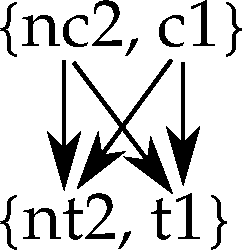
\includegraphics[width=0.35\textwidth]{gfx/ex3.pdf}
		\caption{Graphical error model construction from \textit{panc} to \textit{pant}}
		\label{e3}
	\end{figure}
	
	The figure \ref{e3} clearly shows the set mappings done by the for loop. They correspond to the same index, one index ahead and one index behind from the first set to the second set.
	
	Thus the graph constructed is, $\left\lbrace \textit{nc2} \rightarrow  \textit{nt2}, \textit{nc2} \rightarrow  \textit{t1}, \textit{c1} \rightarrow  \textit{nt2}, \textit{c1} \rightarrow  \textit{t1} \right\rbrace$.
	Intuitively, this graph depicts that the last letter should have been \textit{t}.
	
	\textbf{Example 4, Swapping error:} For the misspelled word \textit{sieze} and the correct word \textit{seize}, we have:
	\begin{equation*}
	\begin{aligned}
	C &= \left\lbrace \textit{1s, 2se, 3ei, iz3, ze2, e1} \right\rbrace \\
	I &= \left\lbrace \textit{1s, 2si, 3ie, ez3, ze2, e1} \right\rbrace \\
	C \cap I &= \left\lbrace \textit{1s, ze2, e1} \right\rbrace \\
	C - C \cap I &= \left\lbrace \textit{2se, 3ei, iz3} \right\rbrace \\
	I - C \cap I &= \left\lbrace \textit{2si, 3ie, ez3} \right\rbrace
	\end{aligned}
	\end{equation*}
	\begin{figure}[h]
		\centering
		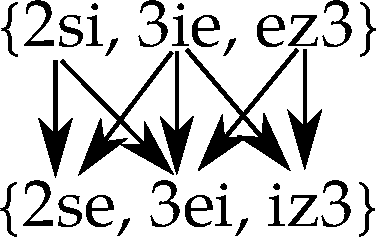
\includegraphics[width=0.5\textwidth]{gfx/ex4.pdf}
		\caption{Graphical error model construction from \textit{sieze} to \textit{seize}}
		\label{e4}
	\end{figure}
	
	Thus the graph constructed is, $\lbrace \textit{2si} \rightarrow  \textit{2se}, \textit{2si} \rightarrow  \textit{3ei}, \textit{3ie} \rightarrow  \textit{2se}, \textit{3ie} \rightarrow  \textit{3ei},$ $ \textit{3ie} \rightarrow  \textit{iz3}, \textit{ez3} \rightarrow  \textit{3ei}, \textit{ez3} \rightarrow  \textit{iz3} \rbrace$.
	Thus the graph neatly captures the idea that the letters \textit{i} and \textit{e} should have been swapped.
	
	\textbf{Example 5, Unequal set length:} For the misspelled word \textit{pth} and the correct word \textit{path}, we have:
	\begin{equation*}
	\begin{aligned}
	C &= \left\lbrace \textit{1p, 2pa, 3at, th2, h1} \right\rbrace \\
	I &= \left\lbrace \textit{1p, 2pt, th2, h1} \right\rbrace \\
	C \cap I &= \left\lbrace \textit{1p, th2, h1} \right\rbrace \\
	C - C \cap I &= \left\lbrace \textit{2pa, 3at, th2} \right\rbrace \\
	I - C \cap I &= \left\lbrace \textit{2pt} \right\rbrace
	\end{aligned}
	\end{equation*}
	\begin{figure}[h]
		\centering
		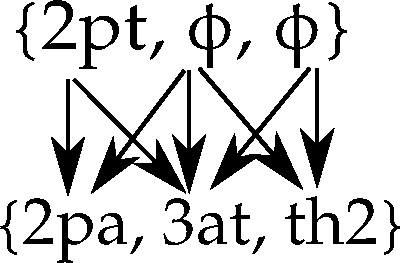
\includegraphics[width=0.5\textwidth]{gfx/ex5.pdf}
		\caption{Directed graph guiding from the incorrect \textit{pth} to the correct \textit{path}}
		\label{e5}
	\end{figure}
	
	Since the size of topmost set was not equal to the bottom one, we inserted empty tokens in the top one unless they become of equal sizes.
	Thus the graph constructed is, $\lbrace \textit{2pt} \rightarrow  \textit{2pa}, \textit{2pt} \rightarrow  \textit{3at}, \phi \rightarrow  \textit{2pa}, \phi \rightarrow  \textit{3at} \rbrace$.
	Thus the graph roughly conveys the information that the letter \textit{t} should be second last.
	
	\textbf{Example 6, Unequal set length:} For the misspelled word \textit{patthhs} and the correct word \textit{paths}, we have:
	\begin{equation*}
	\begin{aligned}
	C &= \left\lbrace \textit{1p, 2pa, 3at, th3, hs2, s1} \right\rbrace \\
	I &= \left\lbrace \textit{1p, 2pa, 3at, 4tt, th4, hh3, hs2, s1} \right\rbrace \\
	C \cap I &= \left\lbrace \textit{1p, 2pa, 3at, hs2, s1} \right\rbrace \\
	C - C \cap I &= \left\lbrace \textit{th3} \right\rbrace \\
	I - C \cap I &= \left\lbrace \textit{4tt, th4, hh3} \right\rbrace
	\end{aligned}
	\end{equation*}
	\begin{figure}[h]
		\centering
		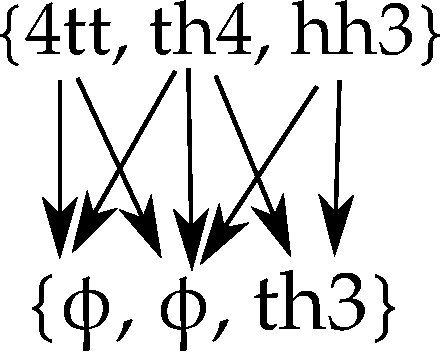
\includegraphics[width=0.5\textwidth]{gfx/ex7.pdf}
		\caption{Graphical error model construction}
		\label{e6}
	\end{figure}
	
	Since the size of bottom set was not equal to the top one, we inserted empty tokens in the bottom set at the middle, unless they become of equal sizes.
	Thus the graph constructed is, $\lbrace \textit{4tt} \rightarrow  \phi, \textit{th4} \rightarrow  \phi, \textit{th4} \rightarrow  \textit{th3}, \textit{hh3} \rightarrow  \phi,  \textit{hh3} \rightarrow  \textit{th3} \rbrace$.
	Thus the graph roughly conveys the information that the letter \textit{t} and letter \textit{h} should have been deleted.
	
	
	In order to evaluate the efficiency of the graphical error model, we will add the probability of each edge of the graph to the score of the ranking function.
	In other words, this would be:
	\begin{equation*}
	\textit{score}(q, d) =  \lambda \times \textit{rank(q, d)} + (1 - \lambda) \times \pi \textit{(q, d)}
	\end{equation*}
	where, $\lambda$ is the weight ranging from $[0, 1]$, \textit{score(q, d)} is the similarity scoring function like BM25 \cite{bm25} or Dirichlet \cite{dirich}  and $\pi \textit{(q, d)}$ is the probabilistic estimate of given error occurring in the training data.
	\begin{equation*}
	\begin{aligned}
	\pi \textit{(q, d)} =  \sum_{g \in G} \textit{count(g)}^s
	\end{aligned}
	\end{equation*}
	Here, $G$ is the constructed graph and $s$ is the strength parameter.
	\textit{count(g)} is the frequency of the error in whole training set of spelling errors.
	We have used $s$ here, to avoid the overfitting during the training, since \textit{count(p)} could heavily depend on the training data.
	
	This function can also be normalized with respect to the cardinality of the pointer set. 
	This could be useful since some of the extremely irrelevant incorrect matches would contain a lot of zeros.
	Thus normalization version, could avoid the skewness of the frequencies.
	
	The normalized version or MAKE is:
	\begin{equation*}
	\begin{aligned}
	\pi \textit{(q, d)} =  \frac{1}{|G|} \sum_{g \in G} \textit{count(g)}^s
	\end{aligned}
	\end{equation*}
% Chapter 3

\chapter{Heuristics on Word Length Similarity} % Chapter title

\label{ch:word} % For referencing the chapter elsewhere, use \autoref{ch:mathtest}

	\section{Guidelines for Feature Engineering in Ranking Functions}

The main idea of the information retrieval systems is to include a proximity score in conjunction to the ranking function. A proximity score is an application-dependent score, like page-rank metrics, contextual similarity and so on. The function should have well engineered feature embedded in itself and it should be able to generalize other results. The objectives of the ranking function are:

\begin{itemize}
	\item The score should be higher if the constituents of proximity score (real numbers or vectors) are similar.
	\item The proximity score should be below certain cut-off scores. These cut-off scores or limiting parameters can be determined through machine learning.
	\item The function should behave similar and able to generalize the behavior and working of the existing ranking functions in IR.
\end{itemize}

The assumption is taken that modeled function is bi-modal (as one has to consider extremities of the cut-off scores). Let $f(\mathbf{x}, \mathbf{y})$ be the modeled function, where $\mathbf{x}$ and $\mathbf{y}$ be the constituent vectors. In other words, this function determines similarity between $\mathbf{x}$ and $\mathbf{y}$ and it is a function of $d(\mathbf{x})$ and $d(\mathbf{y})$ where $d(\cdot)$ is the distance metric.


Length normalization functions, especially in the BM25 or pivoted length function are inversely proportional to the to the TF-IDF score. Thus, the model would be $f(\mathbf{x}, \mathbf{y})$ inversely proportional to the TF-IDF score.


\begin{equation*}
TF-IDF(q, d) \propto \frac{1}{f(\mathbf{x}, \mathbf{y})}
\end{equation*}

\subsection{Nature of the Function Curve}




Since the function has to be bi-modal distribution, distribution function would be modeled in the form asymmetrical inverted bell curve. Thus the trough of the curve should occur when distances of $\mathbf{x}$ and $\mathbf{y}$ are similar. In other words,

\begin{equation} \label{c1}
\frac{\partial f(\mathbf{x}, \mathbf{y})}{\partial ( d(\mathbf{x}) )} = 0 \text{ if } d(\mathbf{x}) \approx d(\mathbf{y})
\end{equation}

Similarly it can be shown that,

\begin{equation*}
\frac{\partial f(\mathbf{x}, \mathbf{y})}{\partial (d(\mathbf{y}))} = 0 \text{ if } d(\mathbf{x}) \approx d(\mathbf{y})
\end{equation*}

From here onwards, arguments would be taken from the $d(\mathbf{x})$ perspective, as $d(\mathbf{y})$ would have similar arguments.

The function should decrease monotonically if $d(\mathbf{x}) < d(\mathbf{y})$. In other words, 

\begin{equation} \label{c2}
\frac{\partial f(\mathbf{x}, \mathbf{y})}{\partial ( d(\mathbf{x}) )} < 0 \text{ if } d(\mathbf{x}) < d(\mathbf{y})
\end{equation}

The function should increase monotonically if $d(\mathbf{x}) > d(\mathbf{y})$. In other words,

\begin{equation} \label{c3}
\frac{\partial f(\mathbf{x}, \mathbf{y})}{\partial ( d(\mathbf{x}) )} > 0 \text{ if } d(\mathbf{x}) > d(\mathbf{y})
\end{equation}

\subsection{Nature of the Limits of the Curve}

Here the left extremity of the curve could be bounded to the parameter $b_1$.
\begin{equation} \label{c4}
\lim_{d(\mathbf{x})\to 0} f(\mathbf{x}, \mathbf{y}) = b_1
\end{equation}

Similarly, the right extremity of the curve could be bounded to the parameter $b_2$.
\begin{equation} \label{c5}
\lim_{d(\mathbf{x})\to \infty} f(\mathbf{x}, \mathbf{y}) = b_2
\end{equation}

The trough of the curve exists when $\frac{\partial f(\mathbf{x}, \mathbf{y})}{\partial ( d(\mathbf{x}) )} = 0$. Thus the limit is set to 1. It can not be set it to 0, because $f(\mathbf{x}, \mathbf{y})$ lies in the denominator of the scoring function.
\begin{equation} \label{c6}
\lim_{d(\mathbf{x})\to d(\mathbf{y})} f(\mathbf{x}, \mathbf{y}) = 1
\end{equation}

The specific case of these guidelines can be applied to the recommendation systems.

%----------------------------------------------------------------------------------------

\section{Design of the TAKE curve}

Here, the function would be modeled using Richard's curve. The curve is defined by,
\begin{equation}
g(x) = l + \frac{u - l}{(A + e^{{-B(x-M)}})^{{1/\nu }}}
\end{equation}

Here, $l$ is lower limit, $u$ is upper limit and $M, \nu, A, B$ are free parameters

The distance metrics are taken to be just real numbers. Thus, $d(\mathbf{x}) = x$ and $d(\mathbf{y}) = y$. The trough of the curve should occur when, $d(\mathbf{x}) = d(\mathbf{y})$ or $x = y$. The function can be partitioned into three parts:
\begin{itemize}
	\item monotonically decreasing Richard's curve, $g(x)$  when $x < y$
	\item monotonically increasing Richard's curve, $g(x)$ when $x > y$
	\item Value of heuristic function, $h(x, y) = 1$  when $x = y$
\end{itemize}

The definition of the function now looks like:

\begin{equation}
h(x, y) = 
\begin{cases}
g(x_1)       & \quad \text{if } x < y\\
1 & \quad \text{if } x = y\\
g(x_2)  & \quad \text{if } x > y\\
\end{cases}
\end{equation}

where $x_1 \in [0, y]$, $x_2 \in [y, \infty]$ and $x_1, x_2 \subset x$

Applying equation (\ref{c1}), the constraint obtained is:

\begin{equation}
\frac{\partial h(x, y)}{\partial x}\at[\bigg]{x=y} = 0
\end{equation}

From equation (\ref{c2}), the constraint obtained is:

\begin{equation*}
\frac{\partial g(x_1)}{\partial x_1} < 0
\end{equation*}

From equation (\ref{c3}), the constraint obtained is:

\begin{equation*}
\frac{\partial g(x_2)}{\partial x_2} > 0
\end{equation*}


From limiting condition (\ref{c4}), the constraint obtained is: 

\begin{align}
\lim_{x_1 \to 0} g(x_1) &= b_1 \\
\frac{\partial g(x_1)}{\partial x_1}\at[\bigg]{x_1 = 0} &\approx 0
\end{align}

From the limiting condition (\ref{c5}), the constraint obtained is: 

\begin{align}
\lim_{x_2 \to \infty} g(x_2) &= b_2 \\
\frac{\partial g(x_2)}{\partial x_2}\at[\bigg]{x_2 = \infty} &\approx 0
\end{align}

From the limiting condition (\ref{c6}), the constraint obtained are: 

\begin{align}
\frac{\partial g(x_1)}{\partial x_1}\at[\bigg]{x_1 = y} &\approx \frac{\partial g(x_2)}{\partial x_2}\at[\bigg]{x_2 = y} &\approx 0  \\
\lim_{x_1 \to y} g(x_1) &= \lim_{x_2 \to y} g(x_2) &= 1 
\end{align}

After solving the constraints, and using the binomial approximation for small $\nu$, the solutions obtained are:

\begin{equation}
h(x, y) = 
\begin{cases}
1 + \frac{b_1 - 1}{1 + e^{B_1(x - cy)}}       & \quad \text{if } x < y\\
1 & \quad \text{if } x = y\\
1 + \frac{b_2 - 1}{1 + e^{-B_2(x - (1 + c)y)}}  & \quad \text{if } x > y\\
\end{cases}
\end{equation}

where,

\begin{itemize}
	\item $B_1$ and $B_2$ are growth parameters, can be typically set to 1
	\item $c$ is the trough curvature, where $c \in (0, 1)$
\end{itemize}

According to the requirements, length similarity would be rewarded between query and document lengths. In that case, $x = |d|$ and $y = |q|$. Intuitively, that means the value of the scoring function will be higher if $|d| \approx |y|$.

Substituting the values, we get:

\begin{equation}
h(|d|, |q|) = 
\begin{cases}
1 + \frac{b_1 - 1}{1 + e^{B_1(|d| - c|q|)}}       & \text{if } |d| < |q|\\
1 &  \text{if } |d| = |q|\\
1 + \frac{b_2 - 1}{1 + e^{-B_2(|d| - (1 + c)|q|)}}  &  \text{if } |d| > |q|\\
\end{cases}
\end{equation}

This feature can now be substituted in the ranking function in place of length normalization function. For example, the original BM25 function is:

\begin{align*}
score(q, d) = & \sum_{t \in d \cap q} f(t, q) \log \frac{M + 1}{df(t)} \times \\
& \frac{ (k + 1) f (t, d) }{f(t, d) + k \left( 1 - b + b \frac{|d|}{avgdl} \right)} 
\end{align*}

The normalization feature $\left( 1 - b + b \frac{|d|}{avgdl} \right)$ in the BM25 formula can be replaced with $h(|d|, |q|)$ to get our desired ranking function:
\begin{equation}
\label{heuris}
\begin{aligned}
score(q, d) = & \sum_{t \in d \cap q} f(t, q) \log \frac{M + 1}{df(t)} \times \\
& \frac{ (k + 1) f (t, d) }{f(t, d) + k \left( h(|d|, |q|) \right)}  \\
\end{aligned}
\end{equation}

\section{Description of TAKE}

The lengths of the misspelled word and correctly spelled word should almost be similar. 
Usually edit distance between misspelled and correctly spelled word are around 1 or 2.
The idea here is to reward the documents more in which document length and query length are closer to each other, and similarly penalize the extremely dissimilar lengths.

Let $|q|$ be the query length and $|d|$ be the document length. Let $h(|q|, |d|)$ be the heuristic function to calculate length similarity. 

The objective of the heuristic function should be:
\begin{enumerate}
	\item $h(|q|, |d|)$ should increase if $|q|$ and $|d|$ are dissimilar
	\item Similarly, $h(|q|, |d|)$ should decrease if $|q|$ and $|d|$ are similar
\end{enumerate}

Here we have used two variants.

\section{Power penalization} This uses hyperparameter $\gamma$ which varies from $[0, 1]$.
\begin{equation}
	\begin{aligned}
		h(|q|, |d|) = (||q| - |d|| + 1)^\gamma
	\end{aligned}
\end{equation}

The nature of the curve is plotted in Figure \ref{natures}.
\begin{figure}[h]
	\centering
	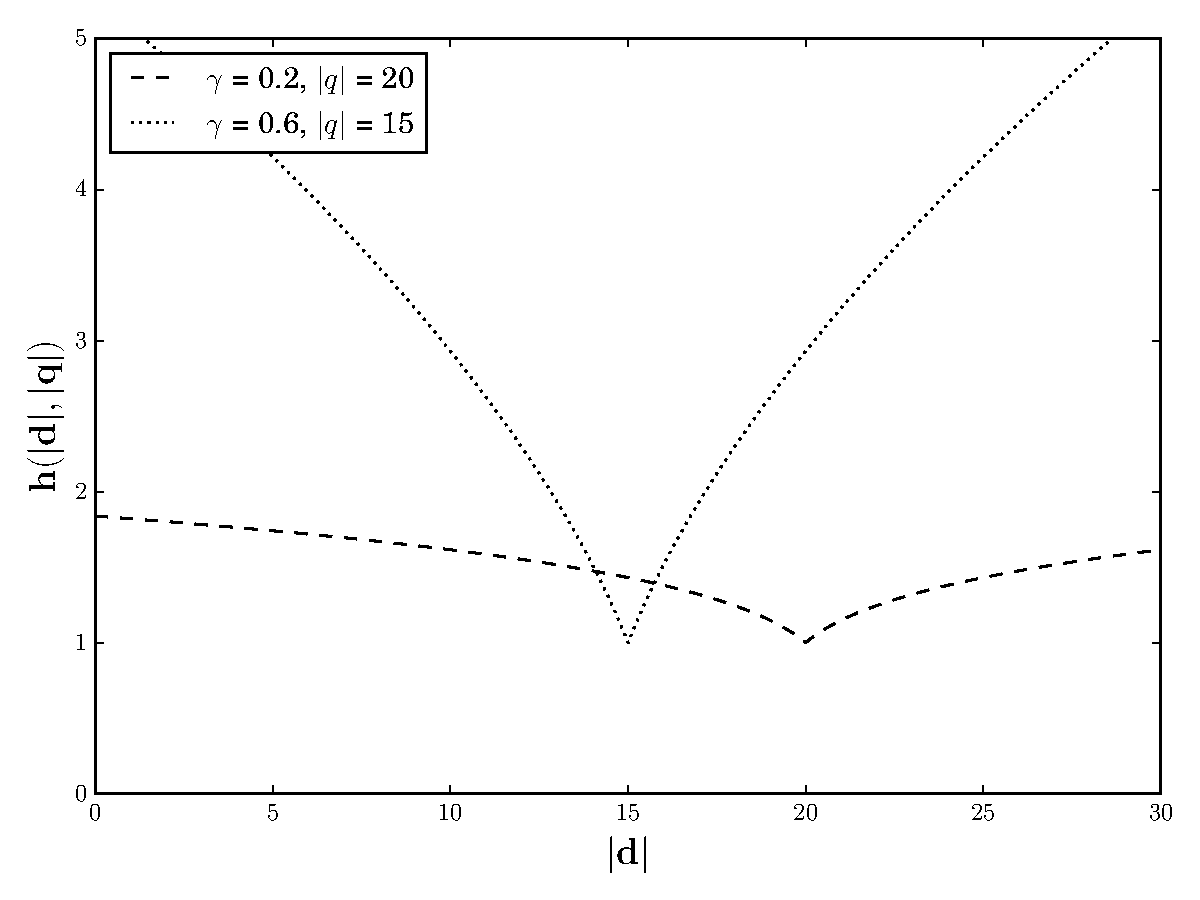
\includegraphics[width=\textwidth]{gfx/test1.pdf}
	\caption{The nature of power penalization $h(|d|, |q|)$ curve. The value of $h(|d|, |q|)$ dips when $|d|$ approaches the $|q|$. As the $\gamma$ increases, penalization would become more harsher.}
	\label{natures}
\end{figure}

\section{Bucket-shaped sigmoidal penalization} 

Here, the function would be modeled using Richard's curve, also known as generalized sigmoidal curve \cite{birch1999new}. 
The curve is defined by,
\begin{equation}
	g(x) = l + \frac{u - l}{(A + e^{{-B(x-M)}})^{{1/\nu }}}
\end{equation}

Here, $l$ is lower limit, $u$ is upper limit and $M, \nu, A, B$ are free parameters

As compared to normal sigmoid function, this function allows more flexibility in the choice of the parameters.
Since, we have to model a penalization function, the aim would be to model a "trough" in the curve as $|q|$ approaches towards $|d|$. 
We divide this function into three parts:

\begin{itemize}
	\item monotonically decreasing Richard's curve, $g(x_1)$  when $|d| < |q|$, or $\frac{\partial g(x_1)}{\partial x_1} < 0$
	\item monotonically increasing Richard's curve, $g(x_2)$ when $|d| > |q|$, or $\frac{\partial g(x_2)}{\partial x_2} > 0$
	\item Value of heuristic function, $h(|d|, |q|) = 1$  when $|d| = |q|$
\end{itemize}

where $x_1 \in [0, |d|]$, $x_2 \in [|d|, \infty]$ and $x_1, x_2 \subset |q|$. If we solve the limiting derivatives, use binomial approximations and remodel our parameters, we get the following penalization function:

\begin{equation}
	h(|d|, |q|) = 
	\begin{cases}
		1 + \frac{b_1 - 1}{1 + e^{B_1(|d| - c|q|)}}       & \text{if } |d| < |q|\\
		1 &  \text{if } |d| = |q|\\
		1 + \frac{b_2 - 1}{1 + e^{-B_2(|d| - (1 + c)|q|)}}  &  \text{if } |d| > |q|\\
	\end{cases}
\end{equation}

where, 

\begin{itemize}
	\item $b_1$ is the upper limit on the left side
	\item $b_2$ is the upper limit on the right side
	\item $B_1$ and $B_2$ are growth parameters, can be typically set to 1
	\item $c$ is the trough curvature, where $c \in (0, 1)$
\end{itemize}

The nature of this feature can be plotted as shown against various parameters (Figure \ref{nature}).

\begin{figure}[h]
	\centering
	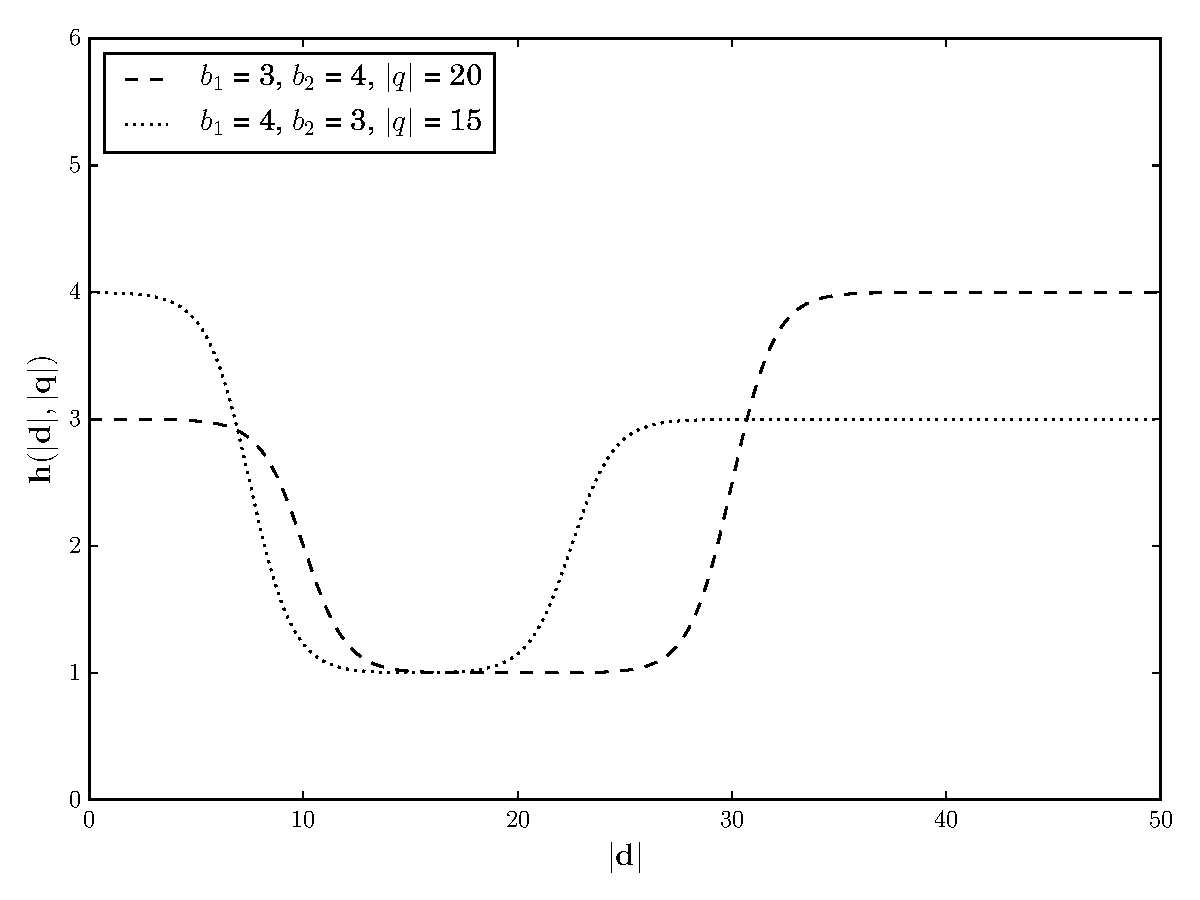
\includegraphics[width=\textwidth]{gfx/test.pdf}
	\caption{The nature of sigmoidal curve $h(|d|, |q|)$ with $B_1 = 1$, $B_2 = 1$ and $c = 0.5$}
	\label{nature}
\end{figure}

If we observe the graph we see a neat bucket-shaped trough when $|d|$ approaches $|q|$. It does not penalizes when the lengths are almost similar but starts penalizing when they are extremely dissimilar. This is feasible as a misspelling (query length) would be around the length of the correct spelling (document length). Using harsh penalization when lengths are dissimilar can prune unnecessary spelling matches with this heuristic.

Clearly, these two penalization heuristics could do behave and achieve the stated objectives. We now demonstrate how we can use this penalization heuristics in our ranking functions.

We know that BM25 ranking function is given by:

\begin{align*}
	score(q, d) = & \sum_{t \in d \cap q} f(t, q) \log \frac{M + 1}{df(t)} \times \\
	& \frac{ (k + 1) f (t, d) }{f(t, d) + k \left( 1 - b + b \frac{|d|}{avgdl} \right)} 
\end{align*}

where $f(t, q)$ is the frequency of terms in queries, $M$ is the number of documents, $k$ is a hyperparameter which sets the bound, $f(t, d)$ is the frequency of terms in documents, $df(t)$ is the document frequency, $b$ is the normalization parameter, $|d|$ is the document length and $avgdl$ is the average document length.

Here $\left( 1 - b + b \frac{|d|}{avgdl} \right)$ is the normalization heuristic. If we replace that heuristic with $h(|d|, |q|)$ we get:
\begin{equation}
	\label{heuris}
	\begin{aligned}
		score(q, d) = & \sum_{t \in d \cap q} f(t, q) \log \frac{M + 1}{df(t)} \times \\
		& \frac{ (k + 1) f (t, d) }{f(t, d) + k \left( h(|d|, |q|) \right)}  \\
	\end{aligned}
\end{equation}

If the value of $h(|d|, |q|)$ decreases, that is if $|d|$ and $|q|$ are similar, then the value of the $score(q, d)$ increases. This means similar document and query word lengths are rewarded. Vice versa can be said if the value of $h(|d|, |q|)$ increases.



We setup an experiment similar to section \ref{experim}, to analyze the behavior of these heuristics on the spelling dataset.
Here we vary $h(|d|, |q|)$ heuristic variants to evaluate their performances.
The results of the experiment are summarized in Table \ref{simexp}.

	Clearly, we see that sigmoidal penalty outperforms the other variants. 
However, sigmoidal penalization function is difficult to train due to large number of parameters.
Hence, we would only consider power penalization for the other experiments. 
\chapter{Experimental Setup} % Chapter title
%
\label{ch:experiment}
We will evaluate our heuristics over three problems: isolated spelling correction, cognate detection and SNP detection.
All of the hyperparameters of baselines presented in this section are tuned in the mentioned datasets according to their best performances.
MeTA toolkit \cite{massung2016meta} is employed to build the search engine.

\section{Spelling Correction}

This problem would be tested using four different datasets:

\begin{enumerate}
	\item \textbf{Conventional English Spelling Evaluation (CESE)}: A collection of 4000 misspellings and their corrections were organized from Fawthrop's contribution in Birkbeck and Wikipedia spelling error corpus \cite{mitton1985birkbeck,wikipedia2017}. 
	These datasets are considered as the gold standard and are commonly tested by other researchers in the spelling correction. 
	The dataset is divided into two parts: training set (comprises of 3000 words) and test set (comprises of 1000 words).
	
	\item \textbf{Low Training Set Evaluation (LTSE)}: We simulated 50000 English misspellings probabilistically. 
	This dataset was then divided into two parts: training set (comprises of 5 words) and test set (comprises of 49995 words). 
	This dataset is constructed to assess how algorithm behaves with less training data (LT).
	
	\item \textbf{Corrupted Label Evaluation (CLE)}: We simulated 50000 English misspellings probabilistically. 
	This dataset was then divided into two parts: training set (comprises of 40000 words) and test set (comprises of 10000 words). 
	From the 40000 words, we mislabeled 20000 of them randomly.
	This dataset is constructed to check the robustness of the algorithms.
	
	\item \textbf{Hindi Spelling Evaluation (HSE)}: A collection of 5000 Hindi errors were taken (error corpus constructed by ourselves). 
	The dataset is divided into two parts: training set (comprises of 4000 words) and test set (comprises of 1000 words). 
	We used the technique called \textit{varn-viched} to tokenize the split the Hindi words into individual k-grams which is analogous to letter splitting technique in Roman languages. 
	
\end{enumerate}

We have chose five baselines for the evaluation purposes : a brute-force looped method \cite{norvig2007write}, weighted longest common subsequence \cite{islam2009real}, finite state transducer \cite{pirinen2010finite}, basic split-up (BREAK-0) with Jaccard similarity and skip-grams \cite{jarvelin2007s}.

\begin{table}[htp]
	\centering
	
	\caption{Test dataset MRR results for spelling correction evaluation}
	\resizebox{0.7 \textwidth}{!}{%
		\begin{tabular}{@{}l|llll@{}}
			\toprule
			\multicolumn{1}{c|}{\textbf{Algorithm Applied}} & \multicolumn{1}{c}{\textbf{CESE}} & \multicolumn{1}{c}{\textbf{LTSE}} & \multicolumn{1}{c}{\textbf{CLE}} & \multicolumn{1}{c}{\textbf{HSE}} \\ \midrule
			Brute-force \cite{norvig2007write} & 68\% & 70\% & 71\% & 38\% \\
			LCS \cite{islam2009real} & 61\% & 59\% & 52\% & 23\% \\
			FST \cite{pirinen2010finite} & 81\% & 22\% & 19\% & 31\% \\
			BREAK-0 + Jaccard & 63\% & 68\% & 67\% & 35\% \\
			Skip-grams \cite{jarvelin2007s} & 65\% & 70\% & 68\% & 29\% \\ \midrule
			BREAK-0 + Dirichlet & 70\% & 65\% &  69\% & 66\% \\
			BREAK-0 + BM25 & 69\% & 70\%  & 68\% & 64\% \\
			BREAK-2 + Dirichlet & 72\% & 72\% & 69\% & 68\% \\
			BREAK-2-Off + Dirichlet & 75\% & 76\% & 71\% & 70\% \\
			BREAK-2 + TAKE + BM25 & 78\% & \textbf{79\%} & \textbf{74\%} & 75\% \\
			BREAK-2 + TAKE + MAKE + BM25 & \textbf{86\%} & 38\% & 35\% & \textbf{84\% }\\ \bottomrule
		\end{tabular}%
	}
	\label{spell-table}
\end{table}


We used MRR (Mean Reciprocal Rank) here as our evaluation metric, since each misspelling had only one solution in our dataset. 
Aspell \cite{atkinson_2016} with the dictionary size of 60 has been used to create the spell-check dictionary for the English evaluation. 

The results in Table \ref{spell-table} show that BREAK-2 with BM25 based length penalty (TAKE) and graphical error models (MAKE) performed the best in conventional English and Hindi spelling evaluation. 
BREAK-2 combined with the BM25 based length penalty (MAKE) performed the best in the corrupted label and low training dataset size evaluation, as these techniques are robust against data abnormalities.


\section{Cognate Detection}

This experiment was performed on the dataset and evaluation scheme proposed by Taraka \cite{rama2015automatic}.
In this dataset, the word pairs are organized into cognate class numbers. 
Positive and negative labels are assigned to the same and different class numbers respectively.
For comparisons, we chose SVM classifier for cognates detection as proposed by Houndrak et al. \cite{kondrak2006evaluation} and Naive Bayes based features as proposed by Alina et al. \cite{ciobanu2014building}
The dataset was divided in the ratio of 3:1 for the training and testing purposes.

\begin{table}[htp]
	\centering
	\caption{Test dataset results for cognate detection experiment}
	\resizebox{0.6 \textwidth}{!}{%
		\begin{tabular}{@{}l|ll@{}}
			\toprule
			\multicolumn{1}{c|}{\textbf{\textbf{Algorithm Applied}}} & \multicolumn{1}{c}{\textbf{P@1}} & \multicolumn{1}{c}{\textbf{F1}} \\ \midrule
			Naive Bayes \cite{ciobanu2014building} & 0.75 & 0.4 \\
			SVM \cite{kondrak2006evaluation} & 0.78 & 0.46 \\ \midrule
			BREAK-2-Off + Dirichlet & 0.76 & 0.42 \\
			BREAK-2 + MAKE + TAKE + BM25 & \textbf{0.80} & \textbf{0.48} \\ \bottomrule
		\end{tabular}%
	}
	\label{cognate-table}
\end{table}

Precision at $k = 1$ and F1 scores are used to evaluate the algorithms used in this experiment.
The results in Table \ref{cognate-table} show that BREAK-2 with MAKE and TAKE performed slightly better than the other results.

\section{SNP Detection}

This is a new problem for detecting SNPs (single-nucleotide polymorphism) which corresponds to genetic mutant identification suggested by Nguyen et al \cite{nguyen2016multiple}.
For this experiment, we simulated two datasets.
The dataset D1 contained 10000 genomes. 
Each genome sequence comprises length of 500-600 base pairs for the artificial DNA sequences. 
10 distinct mutations were created for each genome sequence. 
Then the dataset was populated with $99 \%$ noise, resulting in total size of D1 as 1 million genome sequences.
The dataset D2 had 50000 protein sequences with length around 1000-1500 base pairs, which was populated with $99.9 \%$ noise, resulting in total size of D2 as 1.5 million protein sequences. 
The D2 dataset was artificially created with simulating the random patterns and mutations caused by the 21 proteins.
The BREAK-0 with Jaccard similarity is chosen as a baseline and we used MinDist proximity heuristic clubbed with BM25 and BREAK-0 \cite{tao2007exploration}, to compare our results.
\begin{table}[htp]
	\centering
	\caption{Results for gene mutant detection simulation experiment}
	\resizebox{0.9 \textwidth}{!}{%
		\begin{tabular}{@{}l|llll@{}}
			\toprule
			\multicolumn{1}{c|}{\textbf{Algorithm}} & \multicolumn{1}{c}{\textbf{D1 (MRR)}} & \multicolumn{1}{c}{\textbf{D1 (NDCG)}} & \textbf{D2 (MRR)} & \textbf{D2 (NDCG)} \\ \midrule
			BREAK-0 + Jaccard & 0.33 & 0.16 & 0.31 & 0.12 \\
			MinDist + BM25 + BREAK-0  & 0.55 & 0.40 & 0.49 & 0.38 \\ \midrule
			BREAK-n + Dirichlet & 0.99 & 0.98 & 0.95 & 0.94 \\ \bottomrule
		\end{tabular}%
	}
	\label{mutation-table}
\end{table}

MRR and NDCG (Normalized Discounted Cumulative Gain) are used as metrics for our experiment. 
Table \ref{mutation-table} shows that BREAK-n with Dirichlet outperformed others. 
We used 41 and 83 anchor points for D1 and D2 respectively which were obtained by experimentation on cross-validation dataset.
This shows that our heuristics are scalable and works well with larger datasets.
\chapter{Analysis of Results} % Chapter title
%
\label{ch:analysis}

\begin{figure}[h]
	\centering
	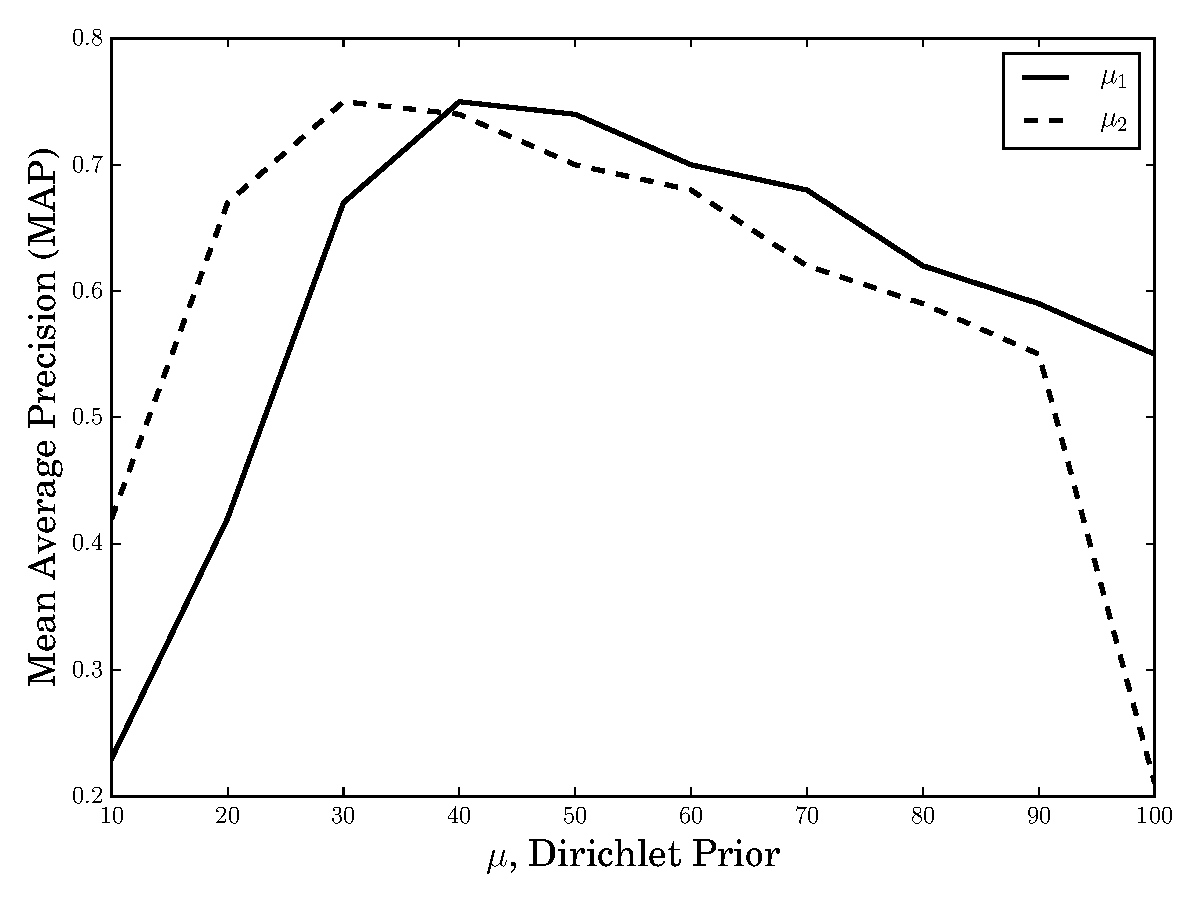
\includegraphics[width=\textwidth]{gfx/phew.pdf}
	\caption{Effect of Dirichlet prior against MAP with BREAK-2 ($\mu_1$) and with MAKE ($\mu_2$)}
	\label{phew}
\end{figure}

Before indexing the documents, the dataset must be split according to the desired BREAK variant.
For the usage of BREAK-n, note that one can store the positional vectors while indexing the corresponding term, or generate the vector directly during evaluation.
This choice highly depends on the time-space tradeoff.
However, in our experiments we have stored the vectors during indexing, prioritizing faster evaluation. 

\section{Analysis of Dirichlet Prior}

The common trend between the experimental setup is that Dirichlet tends to perform better than Okapi BM25.
This is due to the fact that Dirichlet prior smoothing factor, takes account the language modelling, which in turn, makes out to be more successful than vanilla BM25.
We investigate the effect of Dirichlet prior with BREAK-2 $\mu_1$ and with MAKE in $\mu_2$.
Figure \ref{phew} shows that both reach the maximum MAP equally, however $\mu_1$ reaches earlier.

\section{Analysis of Hyperparameters}

Now we analyze the effect of weighted average equation of MAKE, the hyperparameter tuning of the factor $\lambda$.
We investigate the effect of hyperparameter sensitivity in isolated spelling correction $\lambda_1$ and with cognate detection in $\lambda_2$.
\begin{figure}[h]
	\centering
	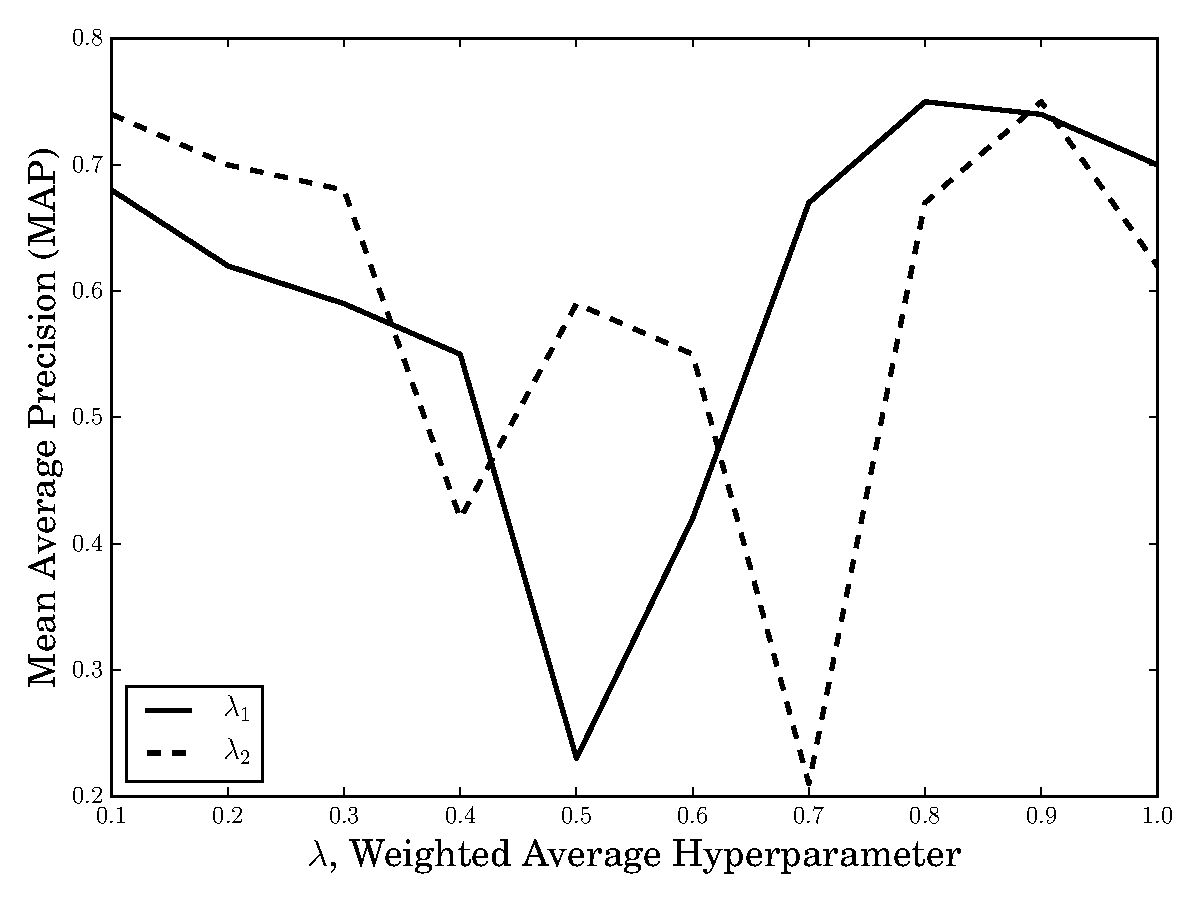
\includegraphics[width=\textwidth]{gfx/phew1.pdf}
	\caption{The effect of hyperparameter sensitivity in isolated spelling correction $\lambda_1$ and with cognate detection in $\lambda_2$.}
	\label{phew1}
\end{figure}

Figure \ref{phew1} describes the optimal conditions of the suitable hyperparameters.
The late reach of $\lambda_2$ suggests that cognate detection experiments depend more on graphical error modelling, MAKE algorithm than the BREAK heuristic.
\chapter{Conclusion} % Chapter title
%
\label{ch:conclusion}

The central theme of this paper is to bring retrieval models and approximate string similarity algorithms together.
We proposed a sequential splitting variants like BREAK-1, 2, Off, n.
To relate these sequential splits, we proposed MAKE algorithm, which constructs the probabilistic distribution between the query and document split sets. 
Finally we designed the TAKE curve, to fit these heuristics in the normalization function of the ranking functions.
In the experiments, we saw that our heuristics were robust against the datasets characteristics like mislabeling, low training dataset size and scales well in larger datasets.
We plan to improve BREAK-n and apply SNP detection problem to real datasets and complex bioinformatics applications in the future.
%

%% Chapter 1
%
\chapter{BREAK: Expansion Sets of Words} % Chapter title
%
\label{ch:expand} % For referencing the chapter elsewhere, use \autoref{ch:name} 
%
A typical text-based search engine system tokenizes queries and documents into words and uses heuristics to return a ranked list of relevant documents to the query.
This analogy can be extended towards string-related operations, where instead of dividing a sentence into words, one could divide a string into small chunks.

The \textit{k-grams} splitting technique illustrates the trivial chunking.
The word \textit{pizza} is split with $k = 2$ as: $\left\lbrace \langle \textit{s} \rangle \textit{p, pi, iz, zz, za, a} \langle / \textit{s} \rangle \right\rbrace$. 
Here, $\langle \textit{s} \rangle$ is the start token and $\langle / \textit{s} \rangle$ is the stop token.
For the sake of the simplicity, we have ignored terminal tokens in the k-gram splits.
Hence, the split set looks like: $\left\lbrace \textit{p, pi, iz, zz, za, a} \right\rbrace$. 
We would label this approach as BREAK-0 because it splits the words into smaller $k$-grams without any sequential information.

\section{BREAK-1: Sequencing from 1 End}
We argue that BREAK-0 could lead to an extremely generalized matching of tokens since an expansion set could be visualized a bag-of-words method. 
Thus, we propose a positional k-gram splitting technique, BREAK-1 which introduces position number in the splits to incorporate the notion of the sequence of the tokens in the word. 
For example, the word \textit{pizza} could be position-wise split with $k = 2$ as: $\left\lbrace \textit{1p, 2pi, 3iz, 4zz, 5za, 6a} \right\rbrace$. 
Thus, the member \textit{4zz} simply means that it is the fourth member of the set.
The motivation behind this tweak is that it gives us a rough amount of sequential-insight for spelling splits when they are used in probabilistic retrieval ranking functions.

\section{BREAK-2: Sequencing from 2 Ends}
The main disadvantage of the BREAK-1 is that some misspellings can easily disturb the order of the set which leads to low similarity.
For example, if the misspelling (query) is \textit{ppizza}, the split set would be $\left\lbrace \textit{1p, 2pp, 3pi, 4iz, 5zz, 6za, 7a} \right\rbrace$.
The order of the members after \textit{2pp} is misplaced, thus this would lead to low similarity with the correct spelling (document) $\left\lbrace \textit{1p, 2pi, 3iz, 4zz, 5za, 6a} \right\rbrace$. 
Only $\left\lbrace \textit{1p} \right\rbrace$ is common between correct and incorrect spell-splits.
Hence, we propose BREAK-2, a split algorithm which is robust against such displacements.

We attach position number to the left if the numbering begins from the start, and to the right if the numbering begins from the end.
Then the smallest position number would be selected between the two position numbers.
If the position numbers are equal, then we select the left position number as a convention.
Figure \ref{algo} gives an exemplification of this algorithm illustrated with splits of \textit{pizza} and \textit{hearts}.

%\begin{figure}[h]
%	\centering
%	\includegraphics[width=0.48\textwidth]{alg.pdf}
%	\caption{The process of BREAK-2. On the left, algorithm slices pizza into pieces. The output set would be $\left\lbrace \textit{1p, 2pi, 3iz, zz3, za2, a1} \right\rbrace$. On the right, algorithm breaks hearts into pieces. The output set would be $\left\lbrace \textit{1h, 2he, 3ea, 4ar, rt3, ts2, s1} \right\rbrace$. }
%	\label{algo}
%\end{figure}
If the misspelling is \textit{ppizza}, the double-end split set would be $\left\lbrace \textit{1p, 2pp, 3pi, 4iz, zz3, za2, a1} \right\rbrace$. 
Thus it gives higher similarity with the correct spelling (document) as compared to positional split, as the set members $\left\lbrace \textit{1p, zz3, za2, a1} \right\rbrace$ would be matched.

\section{BREAK-Off: Sequencing with Offsets} 
We propose another variant, BREAK-\textit{X}-Off, which introduces offsets in the split-sets. 
(Here \textit{X} stands for the BREAK variant number used).
Let the BREAK-1 of pizza be $S_0 = \left\lbrace \textit{1p, 2pi, 3iz, 4zz, 5za, 6a} \right\rbrace$, which has no offsets.
An offset of $1$ would mean the counts would be displaced by 1, which is, $S_1 = \left\lbrace \textit{2p, 3pi, 4iz, 5zz, 6za, 7a} \right\rbrace$.
An offset of -1 would mean the counts would be displaced by -1, which is, $S_{-1} = \left\lbrace \textit{0p, 1pi, 2iz, 3zz, 4za, 5a} \right\rbrace$.
Now the complete split-up would be, thus , $S = S_{-1} \cup S_0 \cup S_1$. 
Similarly, offsets can be applied to the BREAK-2 splits too.

The motivation behind BREAK-\textit{X}-Off is that inclusion of offsets would be robust against the incorrect query provided.
For example, a spelling typographical error could have been caused by the insertion or deletion of the letter. 
Such insertions and deletions would displace the position sequences for the chunks. 
So the key here is to already index these possible errors, like for insertion, it would have an offset of 1 and for deletion, it would have an offset of -1.


\section{BREAK-n: Sequential Splits for Longer Terms}

The main drawback of BREAK-2 algorithm is that the double-ended counts would be inefficient for the longer words. 
With elongation, the advantage of having two extremities would fade away, causing a similar drawback like BREAK-1.
This is undesirable for the non-natural language processing tasks like genome sequence analysis where a typical genetic sequence can be of thousands of base-pairs long.
In this section, we tackle this problem by proposing BREAK-n algorithm, which would generalize BREAK-2 and workaround for longer words.
\subsection{Anchoring}
Here, we introduce the notion of the anchor points.
Notice that in BREAK-2 algorithm, we numbered the terms from two extremities.
Now, instead of 2 extremities here, we number the terms relative to the $n$ extremities or \textit{anchor points}.
For a sequence with a length $l$, divided into $k$-grams and $n$ anchor points, the position of the $i^{th}$ anchor point ($pos_i$) is given by,
\begin{align}
	\label{anchor}
	pos_i = 1 + \frac{(i - 1)(l + k - 1)}{n - 1}
\end{align}
Each anchor point $i$ would have a corresponding vector $t_{e,i}$ having $j$ entries.
Every $t_{e, ij}$ entry will have information about the distance between $i^{th}$ anchor point and their position $j$.
Or simply,
\begin{align}
	\label{relative}
	t_{e, ij} = |pos_i - j|
\end{align}
Here $e$ stands for entity which can be either a document $d$, or query $q$.
%We have illustrated a basic example in figure \ref{breakn} to exemplify this process.
%\begin{figure}[h]
%	\centering
%	\includegraphics[width=0.5\textwidth]{break-n.pdf}
%	\caption{In this example, the words \textit{piza} and \textit{pizza} are given as $q$ and $d$ respectively, split into 2-grams. If we chose 2 anchor points, the position according to equation \ref{anchor} would be at the first and the last (which are shown in arrows). Now we fill every $t_{e, ij}$ entry by calculating relative distance given in equation \ref{relative}.}
%	\label{breakn}
%\end{figure}

\subsection{Redefining Intersection}
Comparing the analogy from BREAK-2, we impose conditional intersection here.
A term $t_q$ in query and $t_d$ in document is said to be \textit{completely intersected} if any of their relative positions from anchor points are same.
To achieve this, we would investigate their column vectors at the matched positions.

Let the matching position for $t_q$ and $t_d$ be $p_1$ and $p_2$, respectively.
We would extract $p_1$ and $p_2$ column vectors and check their corresponding indices for every anchor point.
Afterwards, we extract $p_1$ and $p_2$ column vectors, $t_{q, :p_1}$ and $t_{d, :p_2}$ respectively.
Then we would see if any of their corresponding indices are same.
If this happens, we say that they are \textit{completely intersected}.
In other words, any of the cells in the absolute difference between $t_{q, :p_1}$ and $t_{d, :p_2}$ should be 0.
Mathematically,
\begin{align}
	\label{intersect}
	\prod_{i = 1}^{n} |t_{q, ip_1} - t_{d, ip_2}| = 0
\end{align}
where $n$ is the length of the column vector (number of the anchor points).
If the resulting product around 0 is achieved, we would say that the term intersects completely between query and document.

Continuing the example from figure \ref{breakn}, let's assess the term \textit{za} which is common between $t_q$ ($p_1 = 3$) and $t_d$ ($p_2 = 4$). 
The $t_q$ column vector at $p_1 = 3$ is $t_{q, :3} = [3 \; 1]^T$ and for $t_d$ at $p_2 = 4$ is $t_{d, :4} = [4 \; 1]^T$.
Applying the equation \ref{intersect}, we get $\left(|3 - 4|\right) \left(|1 - 1|\right) = 0$, which means the term \textit{za} is completely intersected.
Analytically, this makes sense because position of \textit{za} from last is same in the two entities, and hence it should be completely intersected.
Although here we have shown the example of BREAK-n for a small word with two anchor points but BREAK-n can be logically extended to longer words with more anchor points.

\section{Combining BREAK with Ranking Functions}
Before indexing the documents, the dataset must be split according to the desired BREAK variant.
For the usage of BREAK-n, note that one can store the positional vectors while indexing the corresponding term, or generate the vector directly during evaluation.
This choice highly depends on the time-space tradeoff.
However, in our experiments we have stored the vectors during indexing, prioritizing faster evaluation. 

We have also combined length penalization heuristics (BREAK-\textit{X}-L) with the probabilistic retrieval functions. 
The role of these heuristics is to reward the documents which are in closer to the length of the query.
This can be useful in the spell correction and cognate detection experiments as misspellings do not much absolute length difference with the correct spelled ones.
These length penalization heuristics can replace the conventional length normalization heuristics which are used in BM25 and Dirichlet.
In addition, we have also introduced graphical error models (BREAK-\textit{X}-G) to analyze the confusion matrix generated during experimentation. 
The motivation behind this creation of graphical error model is to aid the identification and suggestion of solutions to the most probabilistic errors.

%Any misspelled word given as a query and correctly spelled word as a document could make the use of the expansion sets. 
%The word can be broken down into smaller constituents and are indexed accordingly.
%When the misspelling occurs, it is taken as a query, broken down into chunks and searched on the inverted index.
%In this section, we discuss some ways to expand the word into smaller chunks.
%
%\section{Basic k-gram splits}
%This is a well-known way to split the word which is used for spelling correction \cite{Manning:2008:IIR:1394399}.
%The word is split up into \textit{k-grams}.
%For example, the word \textit{pizza} is split with $k = 2$ as: $\left\lbrace \langle \textit{s} \rangle \textit{p, pi, iz, zz, za, a} \langle / \textit{s} \rangle \right\rbrace$. 
%Here, $\langle \textit{s} \rangle$ is the start token and $\langle / \textit{s} \rangle$ is the stop token.
%For the sake of the simplicity, we have ignored tokens in the k-gram splits.
%Hence, the split set looks like: $\left\lbrace \textit{p, pi, iz, zz, za, a} \right\rbrace$.
%
%The other variants include incorporation of skip-grams \cite{jarvelin2007s}, probabilistic distance measures on k-grams \cite{harding1997probabilistic}, usage of similarity scores \cite{damashek1995gauging}, subsequences \cite{islam2009real}, noisy channel models and ranker systems \cite{gao2010large}.
%
%\section{Positional k-gram splits}
%We argue that basic k-gram splits could lead to extreme generalized matching of tokens, since an expansion set could be visualized a bag-of-words model. 
%We introduce positions in the splits to incorporate the notion of sequence of the tokens in the word. 
%For example, the word \textit{pizza} could be position-wise split with $k = 2$ as: $\left\lbrace \textit{1p, 2pi, 3iz, 4zz, 5za, 6a} \right\rbrace$. 
%Thus, the member \textit{4zz} simply means that it is the fourth member of the set.
%The advantage of positional splits can be that it gives us some amount sequential-insight of spelling splits when they are used in probabilistic retrieval ranking functions.
%
%\section{Double-ended k-gram split:}
%The main disadvantage of the positional k-gram split is that any misspelling can easily disturb the order of the set which leads to low similarity.
%For example, if the misspelling (query) is \textit{ppizza}, the split set would be $\left\lbrace \textit{1p, 2pp, 3pi, 4iz, 5zz, 6za, 7a} \right\rbrace$.
%The order of the members after \textit{2pp} is misplaced, thus this would lead to low similarity with the correct spelling (document) $\left\lbrace \textit{1p, 2pi, 3iz, 4zz, 5za, 6a} \right\rbrace$. 
%Only $\left\lbrace \textit{1p} \right\rbrace$ is common between correct and incorrect spell-splits.
%The goal here is to provide split algorithm which is robust against displacements.
%We introduce the double ended split algorithm, which depicts positions from the start as well the end of the spelling. 
%We attach position number to the left if the numbering begins from the start, and to the right if the numbering begins from the end.
%Then the smallest position number would be selected between the two position numbers.
%If the position numbers are equal, then we select the left position number as a convention.
%Figure \ref{algo} gives a pictorial representation of this algorithm illustrated with splits of \textit{pizza} and \textit{hearts}.
%
%\begin{figure}[h]
%	\centering
%	\includegraphics[width=0.48\textwidth]{gfx/alg.pdf}
%	\caption{The process of double-ended split algorithm. On the left, algorithm slices pizza into pieces. The output set would be $\left\lbrace \textit{1p, 2pi, 3iz, zz3, za2, a1} \right\rbrace$. On the right, algorithm breaks hearts into pieces. The output set would be $\left\lbrace \textit{1h, 2he, 3ea, 4ar, rt3, ts2, s1} \right\rbrace$. }
%	\label{algo}
%\end{figure}
%If the misspelling is \textit{ppizza}, the double-end split set would be $\left\lbrace \textit{1p, 2pp, 3pi, 4iz, zz3, za2, a1} \right\rbrace$. 
%Thus it gives higher similarity with the correct spelling (document) as compared to positional split, as the set members $\left\lbrace \textit{1p, zz3, za2, a1} \right\rbrace$ would be matched.
%
%\section{Positional splits with offsets:} Insertion and deletion of letters are fairly common as spelling errors.
%Insertion of an unnecessary letter displaces one position to the right.
%Similarly, deletion of the letter causes displacement of the position to the left.
%In order to introduce insight of displacements in the split sets, we incorporate positional offsets in the split sets.
%For insertion errors, positional offset of $1$ is included.
%This means we would add $1$ offset to every positional number.
%For example, the split set for \textit{pizza} which was originally $\left\lbrace \textit{1p, 2pi, 3iz, 4zz, 5za, 6a} \right\rbrace$, after adding positional offset of $1$ looks like: $\left\lbrace \textit{2p, 3pi, 4iz, 5zz, 6za, 7a} \right\rbrace$.
%Offset with double-ended split-set now looks like $\left\lbrace \textit{2p, 3pi, 4iz, zz4, za3, a2} \right\rbrace$.
%For deletion errors, positional offset of -1 is included.
%For example, the split set for \textit{pizza} after adding positional offset of -1 looks like: $\left\lbrace \textit{0p, 1pi, 2iz, 3zz, 4za, 5a} \right\rbrace$.
%Offset with double-ended split-set now looks like $\left\lbrace \textit{0p, 1pi, 2iz, zz2, za1, a0} \right\rbrace$.
%The complete split-set would include offsets of -1, 0 and 1. 
%Thus, complete split-set of \textit{pizza} now looks like,
%\begin{equation*}
%	\begin{aligned}
%		&\lbrace \textit{0p, 1pi, 2iz, zz2, za1, a0, 1p, 2pi, 3iz,} \\ 
%		&\quad \textit{zz3, za2, a1, 2p, 3pi, 4iz, zz4, za3, a2} \rbrace
%	\end{aligned}
%\end{equation*}
%However, set members $\left\lbrace \textit{0p, a0, 2p, a2} \right\rbrace$ are unlikely to happen as the numbering always starts from 1.
%Hence we can ignore these members.
%The final set is now,
%\begin{equation*}
%	\begin{aligned}
%		C &= \lbrace \textit{1pi, 2iz, zz2, za1, 1p, 2pi, 3iz,} \\ 
%		&\quad \textit{zz3, za2, a1, 3pi, 4iz, zz4, za3} \rbrace
%	\end{aligned}
%\end{equation*}
%where $C$ is the correct split-set. 
%
%Let the misspelling (query) be entered as \textit{piza}. The $I$, incorrect split-set by this method would be:
%\begin{equation*}
%	\begin{aligned}
%		I &= \lbrace \textit{1pi, 2iz, za1, 1p, 2pi,} \\ 
%		&\quad \textit{3iz, za2, a1, 3pi, 4iz, za3} \rbrace
%	\end{aligned}
%\end{equation*}
%Then the match $C \cap I$ is,
%\begin{equation*}
%	\begin{aligned}
%		C \cap I &= \lbrace \textit{1pi, 2iz, za1, 1p, 2pi,} \\ 
%		&\quad \textit{3iz, za2, a1, 3pi, 4iz, za3} \rbrace
%	\end{aligned}
%\end{equation*}
%Thus this method received more number of term matches, $ | C  \cap I | $ than any other methods. Similarly this method can be visualized for other types of spelling errors like insertion of letters.  % Chapter 1

%\cleardoublepage % Empty page before the start of the next part

%------------------------------------------------

%\ctparttext{You can put some informational part preamble text here. Illo principalmente su nos. Non message \emph{occidental} angloromanic da. Debitas effortio simplificate sia se, auxiliar summarios da que, se avantiate publicationes via. Pan in terra summarios, capital interlingua se que. Al via multo esser specimen, campo responder que da. Le usate medical addresses pro, europa origine sanctificate nos se.} % Text on the Part 2 page describing the content in Part 2

%\part{The Showcase} % Second part of the thesis

 % Chapter 3
%% Chapter X

\chapter{Expansion Sets of Words} % Chapter title

\label{ch:expand} % For referencing the chapter elsewhere, use \autoref{ch:name} 

Any misspelled word given as a query and correctly spelled word as a document could make the use of the expansion sets. 
The word can be broken down into smaller constituents and are indexed accordingly.
When the misspelling occurs, it is taken as a query, broken down into chunks and searched on the inverted index.
In this section, we discuss some ways to expand the word into smaller chunks.

%----------------------------------------------------------------------------------------

\section{Section Title}

Content

%------------------------------------------------

\subsection{Subsection Title}

Content

%------------------------------------------------

\subsection{Subsection Title}

Content

%----------------------------------------------------------------------------------------

\section{Section Title}

Content % Chapter 4 - empty template

%\cleardoublepage % Empty page before the start of the next part

%----------------------------------------------------------------------------------------
%	THESIS CONTENT - APPENDICES
%----------------------------------------------------------------------------------------

%\appendix

%\part{Appendix} % New part of the thesis for the appendix

%% Appendix A

\chapter{Appendix Test}

%----------------------------------------------------------------------------------------

\lipsum[13-14]

%----------------------------------------------------------------------------------------

\section{Appendix Section Test}
\lipsum[15]

\graffito{More dummy text}
\lipsum[16]

%----------------------------------------------------------------------------------------

\section{Another Appendix Section Test}
\lipsum[17]

\begin{table}
\myfloatalign
\begin{tabularx}{\textwidth}{Xll} \toprule
\tableheadline{labitur bonorum pri no} & \tableheadline{que vista}
& \tableheadline{human} \\ \midrule
fastidii ea ius & germano &  demonstratea \\
suscipit instructior & titulo & personas \\
\midrule
quaestio philosophia & facto & demonstrated \\
\bottomrule
\end{tabularx}
\caption[Autem usu id]{Autem usu id.}
\label{tab:moreexample}
\end{table}

\lipsum[18]

There is also a useless Pascal listing below: \autoref{lst:useless}.

\begin{lstlisting}[float=b,language=Pascal,frame=tb,caption={A floating example (\texttt{listings} manual)},label=lst:useless]
for i:=maxint downto 0 do
begin
{ do nothing }
end;
\end{lstlisting} % Appendix A
%% Appendix X

\chapter{Appendix Title}

%----------------------------------------------------------------------------------------

% Content begins here % Appendix B - empty template

%----------------------------------------------------------------------------------------
%	POST-CONTENT THESIS PAGES
%----------------------------------------------------------------------------------------

\cleardoublepage% Bibliography

\label{app:bibliography} % Reference the bibliography elsewhere with \autoref{app:bibliography}

\manualmark % Work-around to have small caps also here in the headline
\markboth{\spacedlowsmallcaps{\bibname}}{\spacedlowsmallcaps{\bibname}} % Work-around to have small caps also
%\phantomsection
\refstepcounter{dummy}

\addtocontents{toc}{\protect\vspace{\beforebibskip}} % Place the bibliography slightly below the rest of the document content in the table of contents
\addcontentsline{toc}{chapter}{\tocEntry{\bibname}}

\printbibliography % Bibliography

%\cleardoublepage% Declaration

\refstepcounter{dummy}
\pdfbookmark[0]{Declaration}{declaration} % Bookmark name visible in a PDF viewer

\chapter*{Declaration} % Declaration section text

\thispagestyle{empty}

Put your declaration here.
\bigskip
 
\noindent\textit{\myLocation, \myTime}

\smallskip

\begin{flushright}
\begin{tabular}{m{5cm}}
\\ \hline
\centering\myName \\
\end{tabular}
\end{flushright}
 % Declaration

%\cleardoublepage% Colophon (a brief description of publication or production notes relevant to the edition)

\pagestyle{empty}

\hfill

\vfill

\pdfbookmark[0]{Colophon}{colophon}

\section*{Colophon}

This document was typeset using the typographical look-and-feel \texttt{classicthesis} developed by Andr\'e Miede. The style was inspired by Robert Bringhurst's seminal book on typography ``\emph{The Elements of Typographic Style}''. \texttt{classicthesis} is available for both \LaTeX\ and \mLyX: 

\begin{center}
\url{https://bitbucket.org/amiede/classicthesis/}
\end{center}

\noindent Happy users of \texttt{classicthesis} usually send a real postcard to the author, a collection of postcards received so far is featured here: 

\begin{center}
\url{http://postcards.miede.de/}
\end{center}
 
\bigskip

\noindent\finalVersionString % Colophon

%----------------------------------------------------------------------------------------

\end{document}
